\documentclass[senior]{IPSstyle}

  \Year{2018}
  \Month{February}
  \Author{44161542-3: YUAN JIANG}

  \Title{Cascaded Fully Convolutional Networks for Object Boundary Detection}

  \Advisor{Professor Jinglu HU}

\usepackage{amssymb,amsmath}

\usepackage{mathptmx}
\usepackage{helvet}
\usepackage{courier}
\usepackage{type1cm}

\usepackage{makeidx}
\usepackage{graphicx,subfigure}
\usepackage{multicol}
\usepackage{multirow}
\usepackage[bottom]{footmisc}

\usepackage{mathrsfs}
\usepackage{amssymb,amsmath}
\usepackage{amsfonts}
\usepackage{color}
\usepackage{CJKutf8}

\usepackage{listings}
\usepackage{algorithm,algorithmicx,algpseudocode}
\usepackage[toc,page,title,titletoc,header]{appendix}

\renewcommand{\algorithmicrequire}{\textbf{Input:}}
\renewcommand{\algorithmicensure}{\textbf{Output:}}

  \Abstract{
In computer vision, object boundary is defined as the enclosed set of edge pixels by which an object is tightly surrounded. Given the object boundary, the shapes and locations of the objects in an image can be easily recognized. However, object boundary detection is still a challenging problem due to the multi-scale object problem, the interference caused by the local edges with less semantic information, and the large variance of backgrounds and scenes. In this thesis, we develop a cascaded framework to improve the performance of the present edge detection algorithms in object boundary detection. Within our framework, present networks can be cascaded one-by-one and trained end-to-end to gain more semantic information from the inputs. We test our method in two scenes: neuronal boundary detection in Electron Microscopy (\emph{EM}) images, and object boundary detection in natural images. Massive experiments and analyses show that the proposed cascaded fully convolutional networks can exactly outperform the competitors with the help of the cascaded structure.
}

\Keywords{Fully Convolutional Networks, Object Boundary Detection, Neuronal Segmentation, Cascaded Structures}

\Acknowledgments{

One year ago I chose to leave home and come here with the encouragement from my family, which took the most memorable days in my life to me. So firstly, I would thank my mother and father for their comprehension and supports.

I would express my sincere thinks to Professor Jinglu Hu. Professor Hu is a warm-hearted supervisor who always provides the guidance and suggestions on me, and a rigorous researcher. Without the insightful suggestions and kind reminders from Professor Hu, there might be a hard time for me especially in the days of graduating. 

I would also appreciate Dr. Shen, my supervisor in Shanghai University for teaching me the basic scientific accomplishment and providing me inspirations on the research. 

Thanks my friends who lended me a hand when I went into troubles.

Thank you all!



}


\begin{document}

 \makepreliminarypages
 \singlespace
 \frontmatter
 \tableofcontents
 \listoffigures
 \listoftables
 \mainmatter
 \clearemptydoublepage
 \setlength{\baselineskip}{23.0pt}

\chapter{Introduction} \label{introduction}



\section{Background and Motivation}

\begin{figure}[t]
  \centering
  % Requires \usepackage{graphicx}
  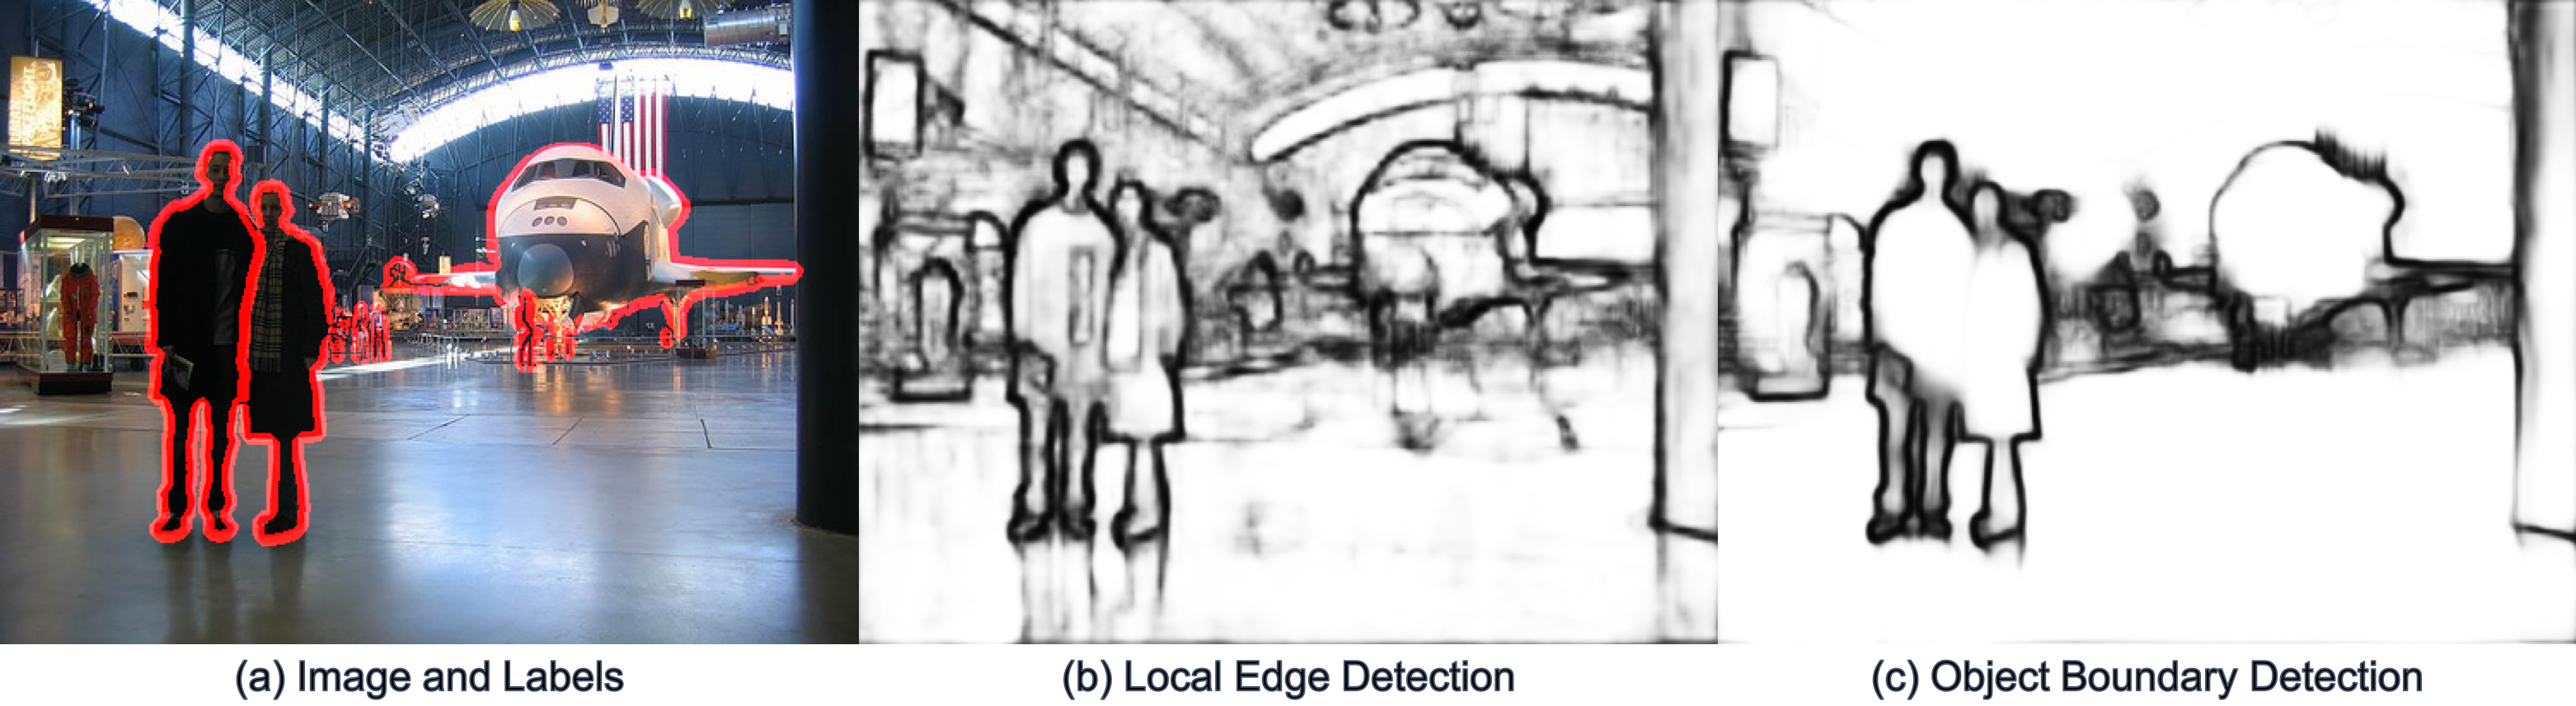
\includegraphics[width=15cm]{object_boundary_vs_local_edge.png}\\
  \caption{Object-level boundary detection is different from the traditional local edge detection, where the former mainly focuses on detecting the high-level semantic boundaries. The first image contains the annotations, which are marked with red lines, for object-level boundary detection.}\label{object_boundary_vs_local_edge}
\end{figure}

Object boundary detection aims at finding the enclosed boundary in which contains an object. Comparing to traditional edge detection, object boundary detection only considers the boundaries related to objects, despite of the low-level edges which have less semantic information (Fig. \ref{object_boundary_vs_local_edge}). So the object boundary can be easily applied for instance-level object segmentation, object proposal\cite{Yang2016, Zitnick2014}, biomedical engineering\cite{Lee2015, Quan2016, Ronneberger2015}, etc. While it is important and useful in various vision tasks, there are few literature about the object boundary detection due to three challenges: First, object boundary detection is a multi-scale problem;  Second, amount of local edges with less semantic information must be inhibited to gain a high-level boundary map; And the large variance of backgrounds and scenes.

Traditional methods mostly focus on extract single-scale features for edge detection\cite{Canny1986, Sobel2014, Dollar2013, Shen2015}. However, objects has various scales in many applications, resulting in the demand of multi-scale descriptors to detect object boundaries. HED\cite{Xie2015} is the first to adopt the supervised multi-scale feature learning to edge detection, where the feature map from each stage of the convolution neural networks is supervised by the ground-truth labels. We follow the multi-scale feature extracting proposed by HED\cite{Xie2015} and extend it to object boundary detection, in which the multi-scale problem is considerably serious.

What's more, the target of traditional edge detection is to identify the discontinuities of image brightness, regardless of the semantic information which indicate whether the edges enclose an object in it. This is the root why some traditional edge detection methods fail to detect the object boundary. We propose the cascaded fully convolutional networks \emph{(FCNs)}\cite{Long2015} with holistic training and testing to overcome the shortages of traditional edge detectors. By recursively connect the FCNs rather than simply stacked the convolution layers, our networks have the ability to inhibit the meaningless edges inside the objects and can be easily interpreted.

Another issue for object boundary detection is the large variance of backgrounds and scenes. Our networks draw inspiration from the related works about neuronal boundary detection in Electron Microscopy \emph{(EM)} images, so we firstly make an effort to apply them on two mainstream datasets for neuronal boundary detection and neuronal segmentation in EM images. To extend the cascaded framework into common cases, we then test our networks in a large natural image dataset, PASCAL Contour\cite{Yang2016}.

We highlight three points in the thesis. (1) extending the multi-scale holistic network of HED\cite{Xie2015} to the multi-scale multi-recursive network for object boundary detection. (2) cascaded network structure with end-to-end training, which is easy to be integrated with other fully convolutional networks. (3) and systematic experiments in two applications to show the reliability and interpretability of our architecture.


%%%%%%%%%%%%%%%%%%%%%%%%%%%%%%%%%%%%%%%%%%%%%%%%%%%%%%%%%%%%%%%%%%%%%%%%%%%%%%%


\section{Application Scenes}

\subsection{EM Images}
With the development of Electron Microscopy \emph{(EM)}, neuroscientists and cognitive scientists are able to study the connection between structures and functions of neurons from the high-resolution EM images\cite{Lichtman2011}. The first step for the study is often to reconstruct the structure of neuronal circuits. However it would take thousands of hours for an expert to annotate a large number of EM images, which motivates researchers to explore some automatic reconstructing algorithms. To reconstruct the neuronal circuits, we firstly reconstruct the 2D structure of neurons from a serials of EM images produced by a serial section EM. Then the stack of 2D neuron structure will be concatenated into the 3D neuron structure. 

As the basic step, 2D neuron reconstruction has drawn a lot of attentions, especially those adopting the powerful deep neural networks\cite{Ciresan2012, Lee2015, Quan2016}. All these approaches convert the reconstruction problem into a 2D boundary detection issue, since the later is easier to be modeled as a binary classification problem and thus there are many literatures and tools can be used to solve it. So long as the neuron boundary is decided, the neuronal circuit can be segmented using simple graph-based methods such as the watershed algorithm\cite{Zlateski2015}. 

Neuronal boundary detection in EM images is a special case of object boundary detection. There are several commons between neuronal boundary detection and object boundary detection, for example, both them focus on the high-level boundary, with less consideration about the low-level local edges. In neuronal boundary detection, to be specific, the low-level local edge includes the ones from background and EM noises, and also the ones produced by confounding structures like nucleus, mitochondria, etc. Hence, traditional edge detectors\cite{Xie2015, Canny1986, Sobel2014} often fail to detect the boundary in EM images (Fig. \ref{object_boundary_vs_local_edge}). Deep neural networks are also widely used to detect neuronal boundary and have gained promising progress\cite{Ciresan2012, Lee2015}, while lack of Multi-recursive-input vs. Single-recursive-input. Different from all these works, we use a lot of experiments not only to show the performance of the proposed cascaded fully convolutional networks in neuronal boundary detection, but also to explain how the proposed architecture removes the insider local edges and background noises, and strengthens the boundary with low-contrast.

We compare our method with competitors on two mainstream datasets for neuronal segmentation, the Piriform dataset\cite{Lee2015} and the ISBI 2012 Challenge dataset\cite{Ronneberger2015}.

\subsection{Natural Images}
Although our idea is firstly motivated by the problem we met in neuronal boundary detection, we also take lots of attentions in extending the proposed models into more commonly used applications, such as the object boundary detection in natural images. Given the object boundary map of a natural image, we can easily obtain the object proposal, object segmentation\cite{Arbelaez2011, Pinheiro2015}, object detection\cite{Everingham2010, Girshick2015}, and recognize object using shape based classification methods\cite{Wang2014, Shen2014CCPR, Shen2016PRL}.

Object boundary detection in natural images is still a difficult problem due to the fact that objects vary in colors, brightness, scales, shapes, textures and gestures. One can hardly recognize the boundaries of all kinds of objects in natural images with only one of the features. Thus, many traditional edge detection methods\cite{Canny1986, Sobel2014} do not perform well when directly applying them for high-level object boundary detection. 

Performance benchmark is done on the famous PASCAL VOC dataset\cite{Everingham2010}. PASCAL VOC is one of the most famous object detection and segmentation challenge held once a year. We collect the training and validation data from PASCAL VOC 2007, to PASCAL VOC 2012. Ground-truth boundary maps are obtained from the instance-level segmentation annotations provided by the official. Comparison results show our cascaded network outperforms not only the traditional edge detectors but also the deep networks without cascade.

%%%%%%%%%%%%%%%%%%%%%%%%%%%%%%%%%%%%%%%%%%%%%%%%%%%%%%%%%%%%%%%%%%%%%%%%%%%%%%%


\section{Organization of the thesis}
The rest of this thesis is structured as follows: Chapter \ref{related_work}  introduces some related works in traditional edge detection methods and neuronal boundary detection methods, concluding their progresses and shortages. In Chapter \ref{methodology}, we describe the proposed cascaded fully convolutional networks, giving an insight into why we design such a architecture and how it works. To evaluate the performance and verify the interpretation, Chapter \ref{experiments} tests our models on three datasets, two for neuronal boundary detection / segmentation in EM images, and one for object boundary detection in natural images. The thesis ends in Chapter \ref{conclusions} with conclusions and future works of this research.

%%%%%%%%%%%%%%%%%%%%%%%%%%%%%%%%%%%%%%%%%%%%%%%%%%%%%%%%%%%%%%Chapter 3
\chapter{Related Work} \label{related_work}
%%%%%%%%%%%%%%%%%%%%%%%%%%%%%%%%%%%%%%%%%%%%%%%%%%%%%%%%%%%%%%Chapter 3


%%%%%%%%%%%%%%%%%%%%%%%%%%%%%%%%%%%%%%%%%%%%%%%%%%%%%%%%%%%%%%%%%%%%%%%%%%%%%%%
Comparing with traditional edge detection, object boundary detection focuses on the high-level semantic information about the objects appeared in the image. It is useful in many applications and has many advantages to the local edges, however, object boundary still lacks of researches in literature. So we will start from traditional edge detection methods to seek the recommendation. On the other hand, neuronal boundary detection in EM images has achieved considerable progresses. Deep neural networks perform well in the neuronal boundary detection, inspiring us to explore a more powerful and explainable one to improve the boundary detection results for not only the EM images, but also the natural images.


\section{Traditional edge detection}

Edge detection is a fundamental task with a long history in computer vision. Contrast to object boundary detection, local edge detection concerns all the pixels with color, brightness, texture, and other properties changing sharply in local parts of an image. 

\subsection{Hand-crafted feature based methods}

Canny\cite{Canny1986} can be seen as the pioneer of computationally extracting edges from digit images. Canny uses image gradient to get the edges. Firstly, the input RGB image should be converted to a greyscale one, whose 2D gradient map will be next calculated using the Sobel\cite{Sobel2014} filters. Then the non-maximum suppression is applied in the gradient map to get the thinned edges. After that Canny proposed to adopt an empirically selected double threshold to filtering the edges, where the edges higher than the high threshold will be marked as the "strong edges", the edges lower than the low threshold will be marked as background, and the rest of edges are so called the "weak edges". Canny descriptor use only the brightness gradient of the image, but has almost no ability to utilize the color and texture information of the image, much less the semantic information.

The followers \cite{Malik2001, Arbelaez2011, Krahenbuhl2015} tend to combine brightness, color and texture gradients to make a better use of RGB inputs. All these methods are patch-based learning methods. In training phase, random sampled mini patches are cropped from original input image. Features of these patches are extracted using various cues mentioned above. Then the features of training samples will be fed into a two-class classifier, such as Support Vector Machine and Random Forest, to judge whether the central pixel of the sample is an edge pixel or not. In test phase, a one-step sliding window will be applied for a dense probability map about edge. To detect edges with more semantic meaning, the \emph{gPb}\cite{Arbelaez2011} computes gradients at different scales, but resulting in a huge increase of computational load. Lim et al.\cite{Dollar2013} rather propose a structured feature learning pipeline for an effective and fast detection.

 All these methods choose hand-crafted features based on local cues, with few design for object-level boundary detection. Experiments in Chapter \ref{experiments} will show their shortages in object boundary detection tasks.

\subsection{Deep learning based methods}

Deep Learning, especially the Convolutional Neural Networks \emph{(CNNs)}, developed rapidly in recent years. The CNNs showed their power firstly in the large-scale object recognition challenges. AlexNet, proposed by Krizhevsky et al.\cite{Krizhevsky2012} in 2012, improved the top-5 rate in ILSVRC-2010 and ILSVRC-2012 competition by around 8\%, which drives researchers' trying {Arbelaez2011}on applying the deep feature extraction for most of the computer vision tasks. VGGNet\cite{Simonyan2014}, GoogLeNet\cite{Szegedy2015} and ResNet\cite{He2016} are the followers of \cite{Krizhevsky2012}. All these works tend to find the ways to train a deeper or wider network so that the abstract object-level feature can be better learned and extracted. In the next years, CNNs are also widely applied for object detection\cite{Girshick2014, Girshick2015, Ren2015}, object segmentation\cite{Pinheiro2015}, and object contour detection\cite{Shen2015, Kivinen2014, Ganin2014}.

Similar to \cite{Lim2013}, Shen et al.\cite{Shen2015} cluster the edge structures into several subclasses and convert the two-class classification task to a multi-class one. By this way, the deep networks are able to learn different model parameters for each subclass, and the results are more interpretable. \cite{Shen2015} utilizes the deep features to capture high-level object information and outperforms all the traditional hand-crafted feature based methods. However, in testing phase, the features extracted by fully connected layer must be fed into a structured random forest classifier\cite{Dollar2013} for the final contour detection result. The two-step learning limits the performance of deep networks. What's more, due to the existing fully connected layers, inputing the original images with various scales is forbidden. So the authors\cite{Shen2015} have to adopt the patch-based training and testing, leading to a low detection speed.

In 2014, Fully Convolutional Networks \emph{(FCNs)}\cite{Long2015} are proposed to handle with the per-pixel annotation problem, such as the object segmentation in the famous PASCAL VOC Challenge\cite{Everingham2010}. Developed from VGGNet, FCNs remove the last fully connected layers of it and replace with 1 \(\times\) 1 convolution layers, which releases the limitation of the input size. A non-parameter deconvolution layer is followed by the last convolution layer to up-sample the low-resolution feature maps into probability maps with same resolution of the input. Finally, after properly cropping, the output probability maps will have the same size with the input. When training, these probability maps can be used to calculate the pixel-wise loss with ground-truth labels. FCNs enable the end-to-end training and testing of CNNs for such a pixel-wise prediction task. With FCNs, the precision and speed will not be restricted by the sliding window scheme. 

Features from different stages of the convolution neural networks have the multi-scale information\cite{Xie2015}. Xie et al.\cite{Xie2015} propose to make a full use of these information by extracting features from each stage of the FCNs, then up-sampling them to the same size with the input, which results in multi-scale outputs called side-outputs. All the side-outputs and the fusion of these side-outputs will contribute on the loss, where both the low-level stages with high resolution but little semantic information, and the high-level stages with low resolution but much semantic information can be trained easilier. Benefited from the holistic training and multi-scale features, HED\cite{Xie2015} achieves great performance in the famous edge detection benchmark, BSDS 500\cite{Arbelaez2011}, improving the F-measure\cite{Arbelaez2011} from 0.756\cite{Shen2015} to 0.782. Note that the F-measure of human being's annotation is 0.8.

\section{Object Boundary Detection in Natural Images}

Although HED\cite{Xie2015} and other edge detection methods\cite{Shen2015, Dollar2013, Arbelaez2011} have achieved considerable success in relatively low-level edge detection, they perform bad when applied for the high-level \emph{"object-only"} boundary detection\cite{Yang2016}. Fully Convolutional Encoder-Decoder Network \emph{(CEDN)}\cite{Yang2016} is the pioneer to distinguish object-level boundary detection from traditional local-level edge detection. CEDN uses VGG-16\cite{Simonyan2014} as the encoder and designs an approximately symmetric but light-weighted decoder. During training, it fixes the model parameters of the encoder and only updates the parameters of the decoder. 

CEDN outperforms all the competitors on the large PASCAL VOC Contour Dataset\cite{Yang2016} in object boundary detection benchmark. However, it still has several problems: 
(1) the encoder network does not benefit from the training data at all; 
(2) to achieve the performance in the leaderboard, it requires all the training data to be processed for 30 times, due to the comparatively deep architecture.

\section{Neuronal Boundary Detection in EM Images}

Neuronal segmentation is the fundamental step to learn the structures of neural cells and analyze the relationship between the structures and the functions\cite{Lichtman2011, Helmstaedter2013, Sporns2005}. In early days, however, it would take an expert with professional knowledge lots of time to recognize the segment of neuronal circuits\cite{Helmstaedter2013} in massive EM images, which motivated researchers to find a automatic algorithm to annotate the neuronal segments. People find the key to the neuronal segmentation is to detect the membranes of the cells, while suppressing the local edges within them\cite{Laptev2012, Kaynig2010, Kumar2010, Seyedhosseini2011}. So that graph-based algorithms such as watershed\cite{Najman1996, Uzunbas2014, Zlateski2015} and graph cut\cite{Boykov2001} can be directly used to convert the boundary to segmentation.

To detect neuronal boundary is to extract membranes in an EM image. In this degree, Neuronal Boundary Detection can be seen as a special case of Object Boundary Detection, where the \emph{"object"} in the former is only the neuron circuit. 

Deep learning based methods are able to meet the demand of different applications, by learning the parameters of not only the classifiers, but also the feature extractors. With the rapid development of deep networks, adopting them into the hard neuronal segmentation tasks becomes popular among researchers. Comparing with traditional hand-designed features, deep features need less experts' knowledge to design the feature extractors and can make a full use of the data, which is proved to be effective in neuronal boundary detection tasks\cite{Ciresan2012, Ronneberger2015, Quan2016, Fakhry2017, Lee2015}.
As the winner of the famous ISBI 2012 EM Segmentation Challenge\cite{Carreras2015}, Ciresan et al.\cite{Ciresan2012} successfully apply the deep neural networks with a stack of \emph{convolution-subsampling} units for membrane pixel detection. Ronneberger et al.\cite{Ronneberger2015} propose U-net, which reuses the features of the layers in the encoder part by merging them with the layers in the decoder part, to detect neuronal boundary and segment EM circuits. With the benefit of fully convolutional network structure and multi-level feature concatenating, U-net shows the efficiency in neuronal segmentation by outperforming the competitors in ISBI 2012 by a large margin. With the proposal of ResNet\cite{He2016} in object recognition and detection, Quan et al.\cite{Quan2016} and Fakhry et al.\cite{Fakhry2017} try to implement the deep residual units in their fully convolutional networks, which is also proved to be effective in neuronal boundary detection issues. 

However, most of these works engraft the state-of-the-art network architectures proposed in other vision works as a \emph{"black-box"} to boost the performance of neuronal boundary detection. It is necessary to seek an interpretable and effective approach, so that it can be theoretically comprehensive and enlighten the relative works in the future.

\begin{figure}[t]
  \centering
  % Requires \usepackage{graphicx}
  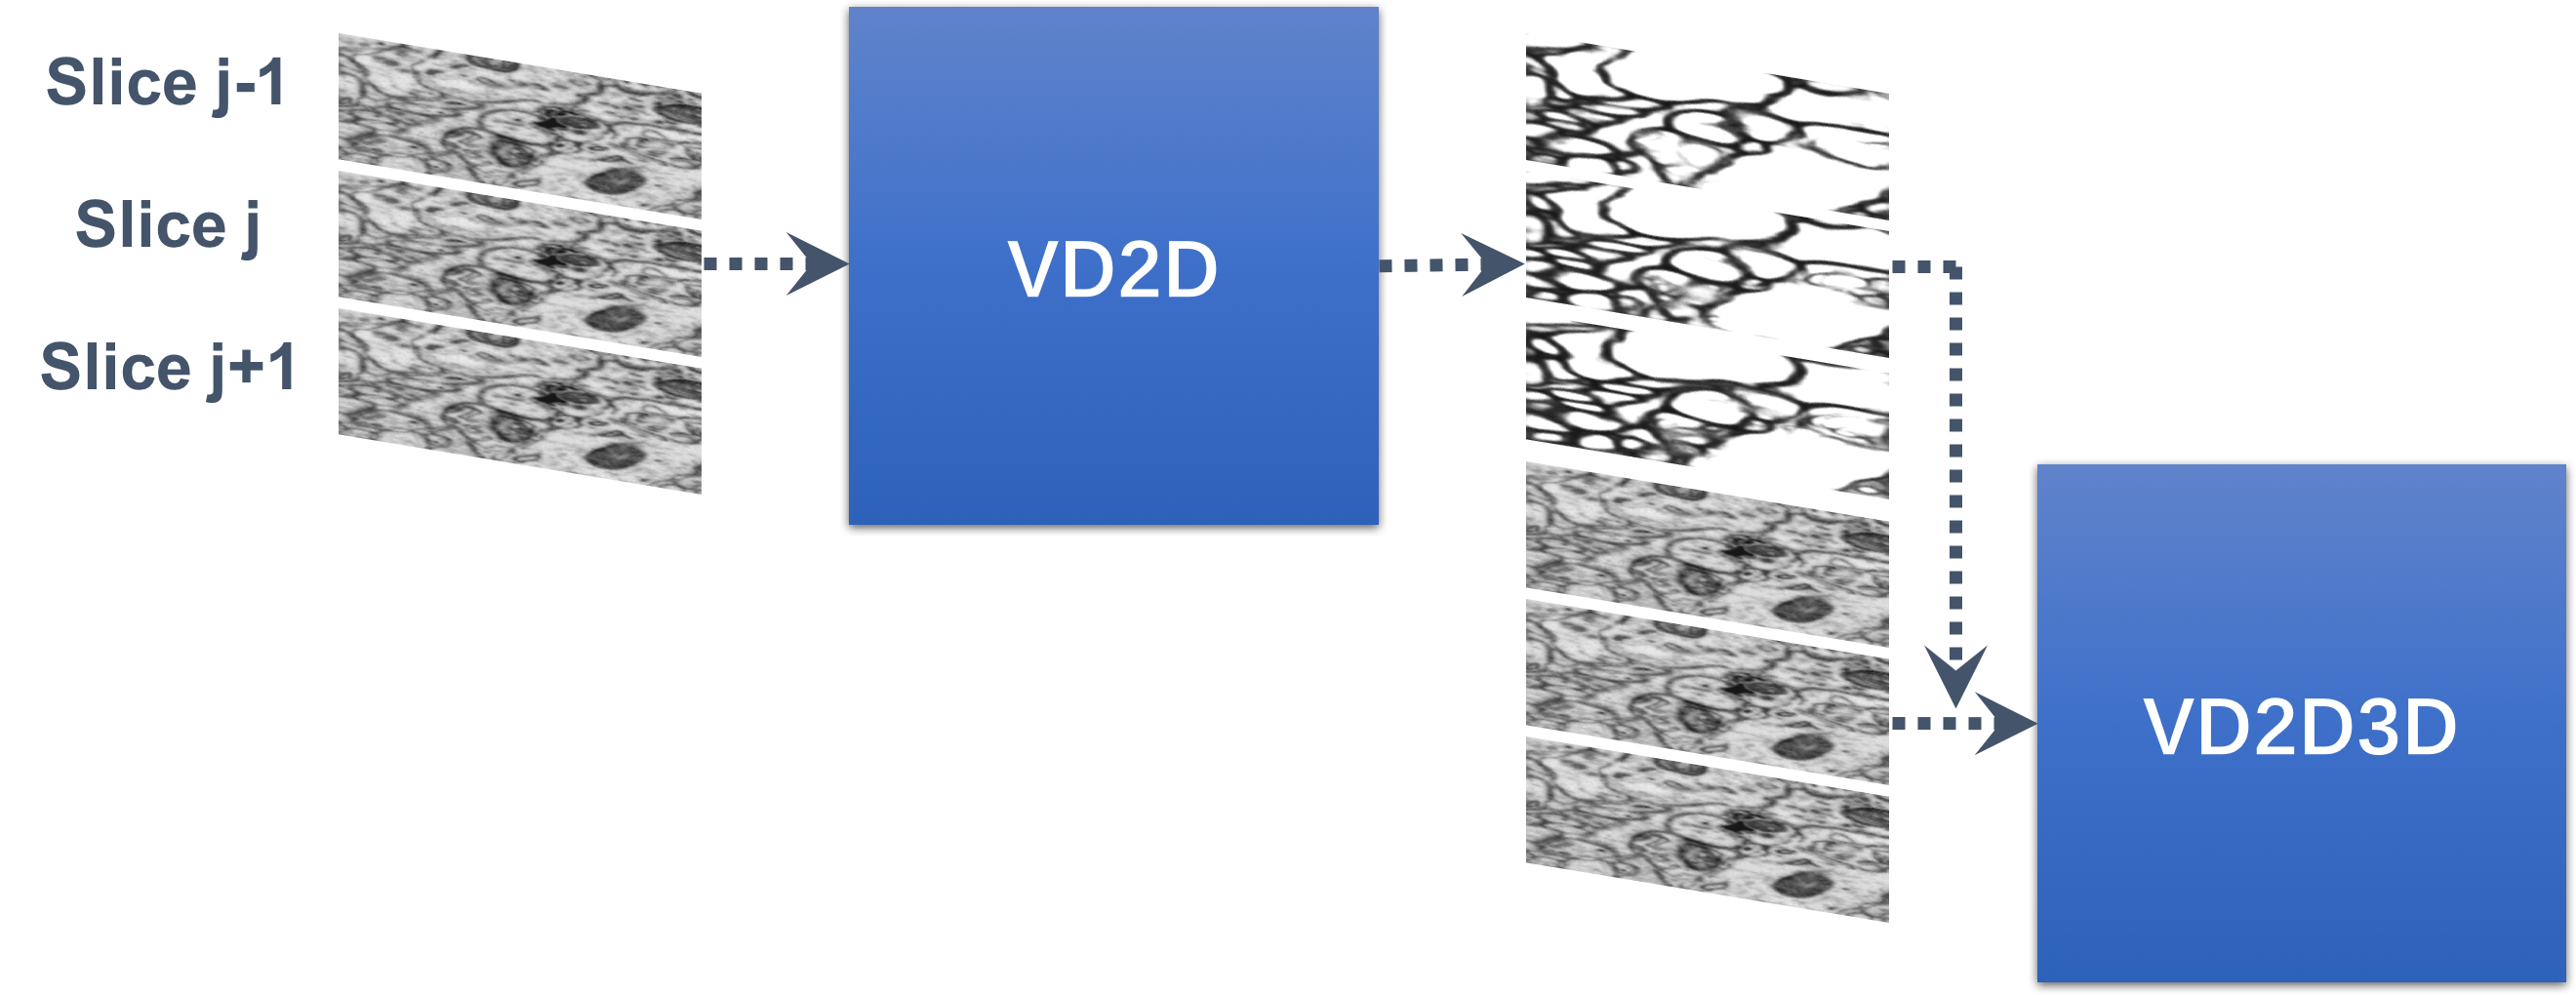
\includegraphics[width=15cm]{vd2d3d.png}\\
  \caption{Illustration of VD2D3D, a recursive deep network with the stepwise training.}\label{Lee2015}
\end{figure}

Most related to our work is Very Deep 2D-3D network \emph{(VD2D3D)} proposed by Lee et al.\cite{Lee2015}. A Very Deep 2D \emph{(VD2D)} network is firstly trained using patches randomly cropped from the images. The model of VD2D will be then used to produce the predictions of a stack of images produced by the serial section EM. \cite{Lee2015} believes the adjacent slices will help to detection the boundary, so VD2D3D concatenates the raw image and the prediction of its adjacent slices, produced by VD2D, as the new training materials of VD2D and recursively fine-tunes last several layers of VD2D.  We find in experiments that \cite{Lee2015} has three main problems: 
(1) it lacks of multi-scale features to better represent the complex neural membranes; 
(2) stepwise training limits the learning ability of the recursive deep networks; 
(3) patch-based testing relies on the sliding window pipeline, which seriously slow down the testing speed. 
Inspired by \cite{Lee2015}, we develop a cascaded fully convolutional network with multi-recursive inputs and train it end-to-end. The proposed network overcomes the shortages of \cite{Lee2015} to achieve the state-of-the-art performance on a neuronal segmentation benchmark\cite{Lee2015} and a large natural object boundary detection benchmark\cite{Ronneberger2015}.

%%%%%%%%%%%%%%%%%%%%%%%%%%%%%%%%%%%%%%%%%%%%%%%%%%%%%%%%%%%%%%%%%%%%%%%%%%%%%%%


\chapter{Methodology} \label{methodology}

In this part, we will introduce the proposed Cascaded Fully Convolutional Networks for object boundary detection. First, the cascaded network structure with multi-recursive inputs is presented. Then we will describe our end-to-end training, where every part of the cascaded network can benefit from the training data. Next, in Section \ref{testing phase}, we will demonstrate how to apply the learned fully convolutional model for the accurate yet fast detection. In the last section of this chapter, we spend a lot of ink to lead you into the insight of the proposed architecture, explaining how it works.

%%%%%%%%%%%%%%%%%%%%%%%%%%%%%%%%%%%%%%%%%%%%%%%%%%%%%%%%%%%%%%%%%%%%%%%%%%%%%%%

\begin{figure}[t]
  \centering
  % Requires \usepackage{graphicx}
  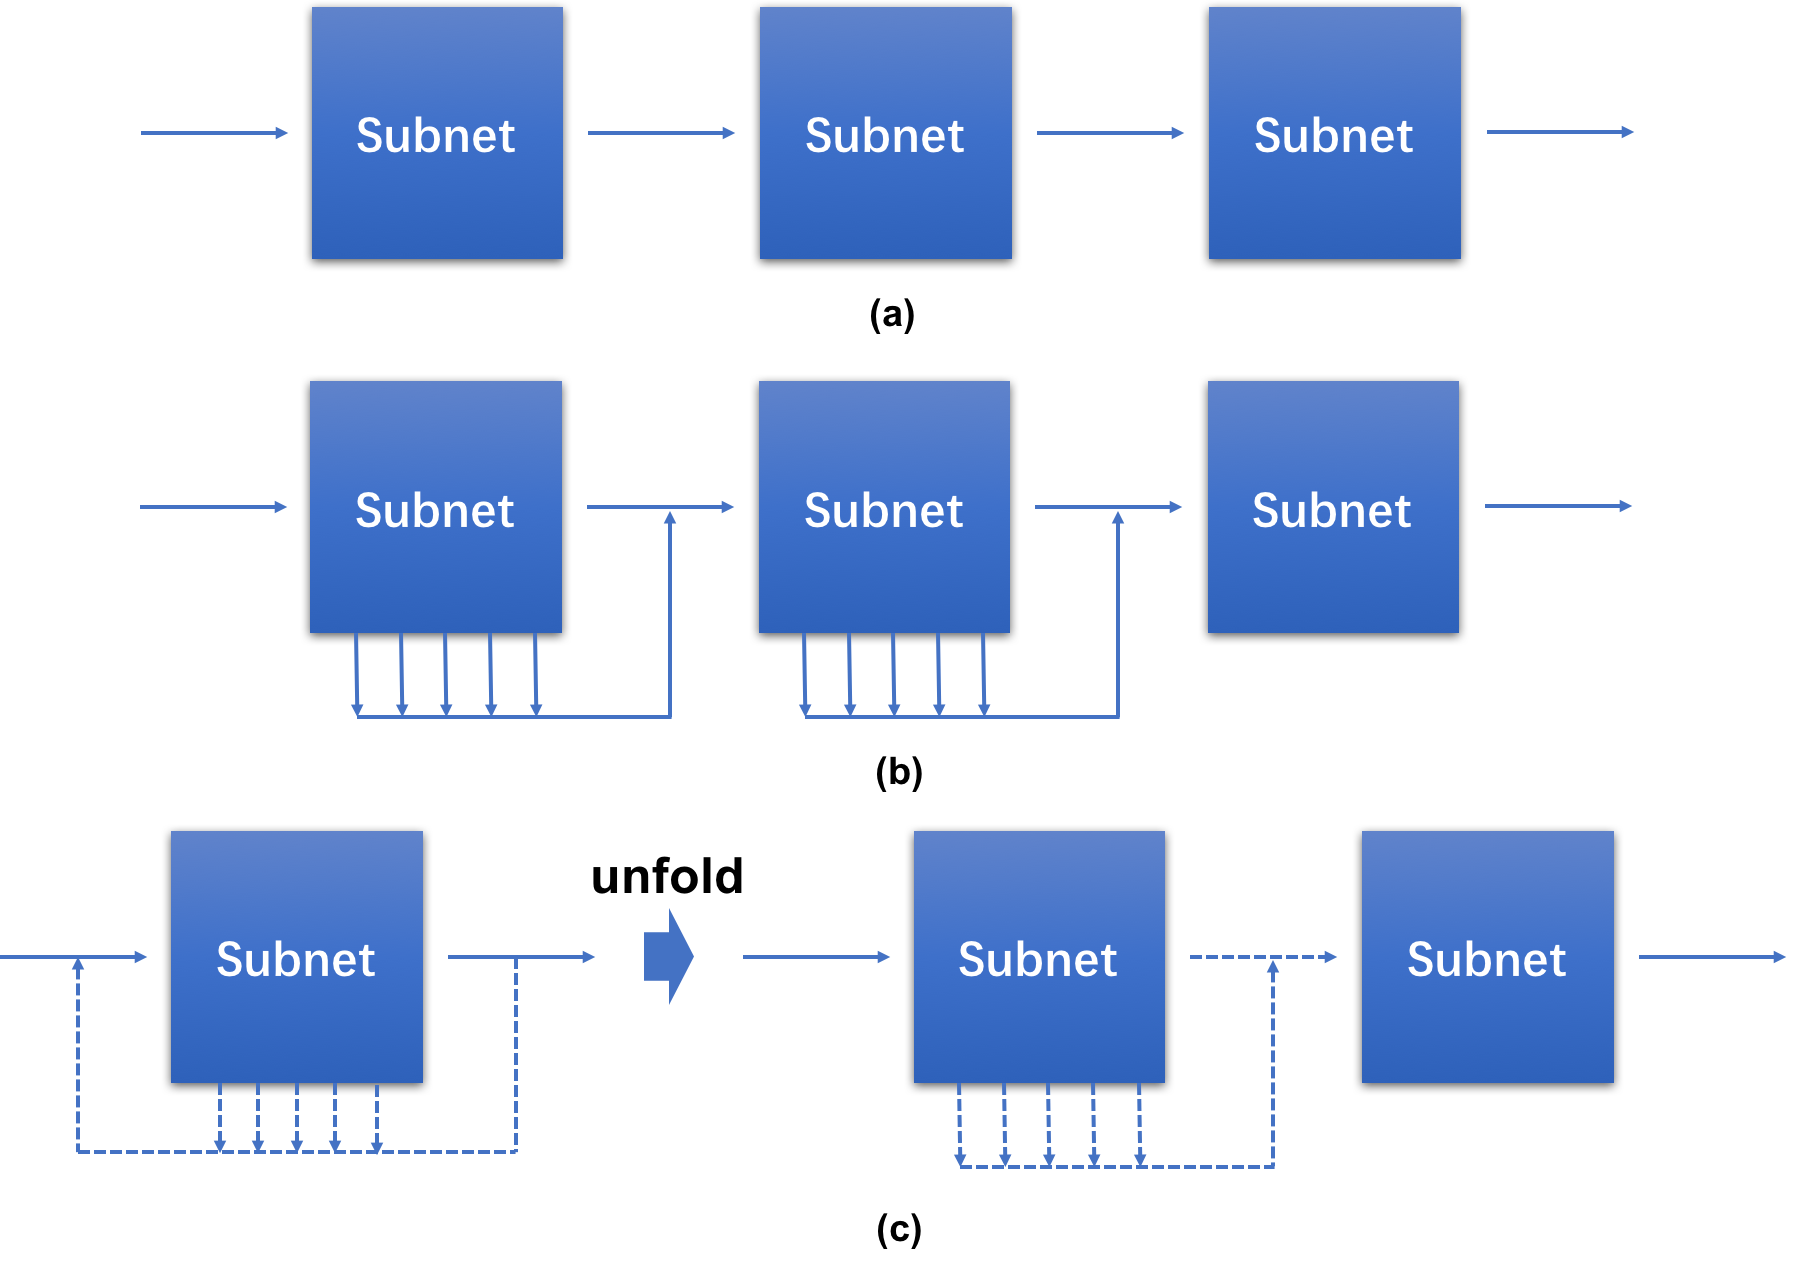
\includegraphics[width=15cm]{cascade_structures.png}\\
  \caption{Three types of cascade-like networks: (a) cascaded network with single-recursive input; (b) cascaded network with multi-recursive inputs; (c) single-stage network with recursive inputs to fine-tune itself.}\label{cascade_structures}
\end{figure}

\section{Network Structure} \label{network structure}

As shown in Fig. \ref{cascade_structures}, we considered several methods to assemble our cascaded networks. Fig. \ref{cascade_structures}(a) shows the structure of single-recursive-input cascaded fully convolutional networks, which feeds the final output of the former sub-network into the next sub-network, recursively. Each of these sub-networks is the fully convolutional network with the same structure but unshared model parameters. Fig. \ref{cascade_structures}(b) illustrates the cascaded structure with multi-recursive inputs, our final choice. In this design, the predictions from not only the last layer but also the side-output layers\cite{Xie2015} will be the recursive inputs of the next stage, so we name it as multi-recursive-input design. With contrary to the single-recursive-input one, the proposed architecture makes the full use of features with multiple scales extracted from the former sub-network. Fig. \ref{cascade_structures}(c) is another design for constructing such a multi-stage network, where there is only one sub-network, but fine-tuned time after time by recursively feeding the  predictions into itself. To unfold the recursive connection of the left side of Fig. \ref{cascade_structures}, we can get the equivalent network as shown in the right side. The unfolded version is much similar to the proposed architecture. However, we train all the parameters of sub-networks jointly in the proposed cascaded network, while Fig. \ref{cascade_structures}(c) fixes the parameters of former sub-networks and only fine-tune the ones of the last sub-networks. Experiments in Chapter \ref{experiments} show our design is more effective and efficient than the others.

To be more specific, our network used in object boundary detection can be illustrated as Fig. \ref{network}. It consists of several stages, three in the default setting, each of which is a fully convolutional network. 
By default, each sub-network is built based on the holistically-nested network\cite{Xie2015}, which is converted from the famous VGG-16\cite{Simonyan2014} network. So the subnet has five stages of the convolution-pooling structure, of which the receptive fields are increased with the stepwise dilated strides. For each level, the side-output is obtained by up-sampling the feature from the last convolution layer of the level and activating it using a sigmoid layer. We mark the side-outputs of level 1 to 5 as \(S_{1}^{(p)}\), \(S_{2}^{(p)}\), \(S_{3}^{(p)}\), \(S_{4}^{(p)}\), \(S_{5}^{(p)}\), respectively, where \(p \in{1, 2, 3}\) denotes the order of the sub-network. 

Benefited from the receptive field sizes increasing, side-outputs are able to capture features in different scales naturally, without input scaling. Multi-scale features are then fused using the 1 \(\times\) 1 convolution filters to produce the final predictions for the stage 1, 2, 3, named \(F^{(1)}\), \(F^{(2)}\), \(F^{(3)}\), respectively. And the best prediction we used in benchmarks is the fusion of \(F^{(1)}\), \(F^{(2)}\) and \(F^{(3)}\). As mentioned above, there are abundant multi-scale information stored in the side-outputs, so we concatenate all the side-outputs with fused prediction and the raw image along with the color channel as the input of the next stage, which called the multi-recursive-input schema. 

We choose HED\cite{Xie2015} as the sub-network in each stage to carry on the multi-scale feature extraction and holistic deep supervision proposed by \cite{Xie2015}. Here, the deep supervision refers to use the ground-truth to supervise the prediction of not only the last output, but also the side-outputs\cite{Xie2015}, which avoids gradient vanishing in some degree and allows shallow layers efficiently learn the parameters from data. 

\begin{figure}[t]
  \centering
  % Requires \usepackage{graphicx}
  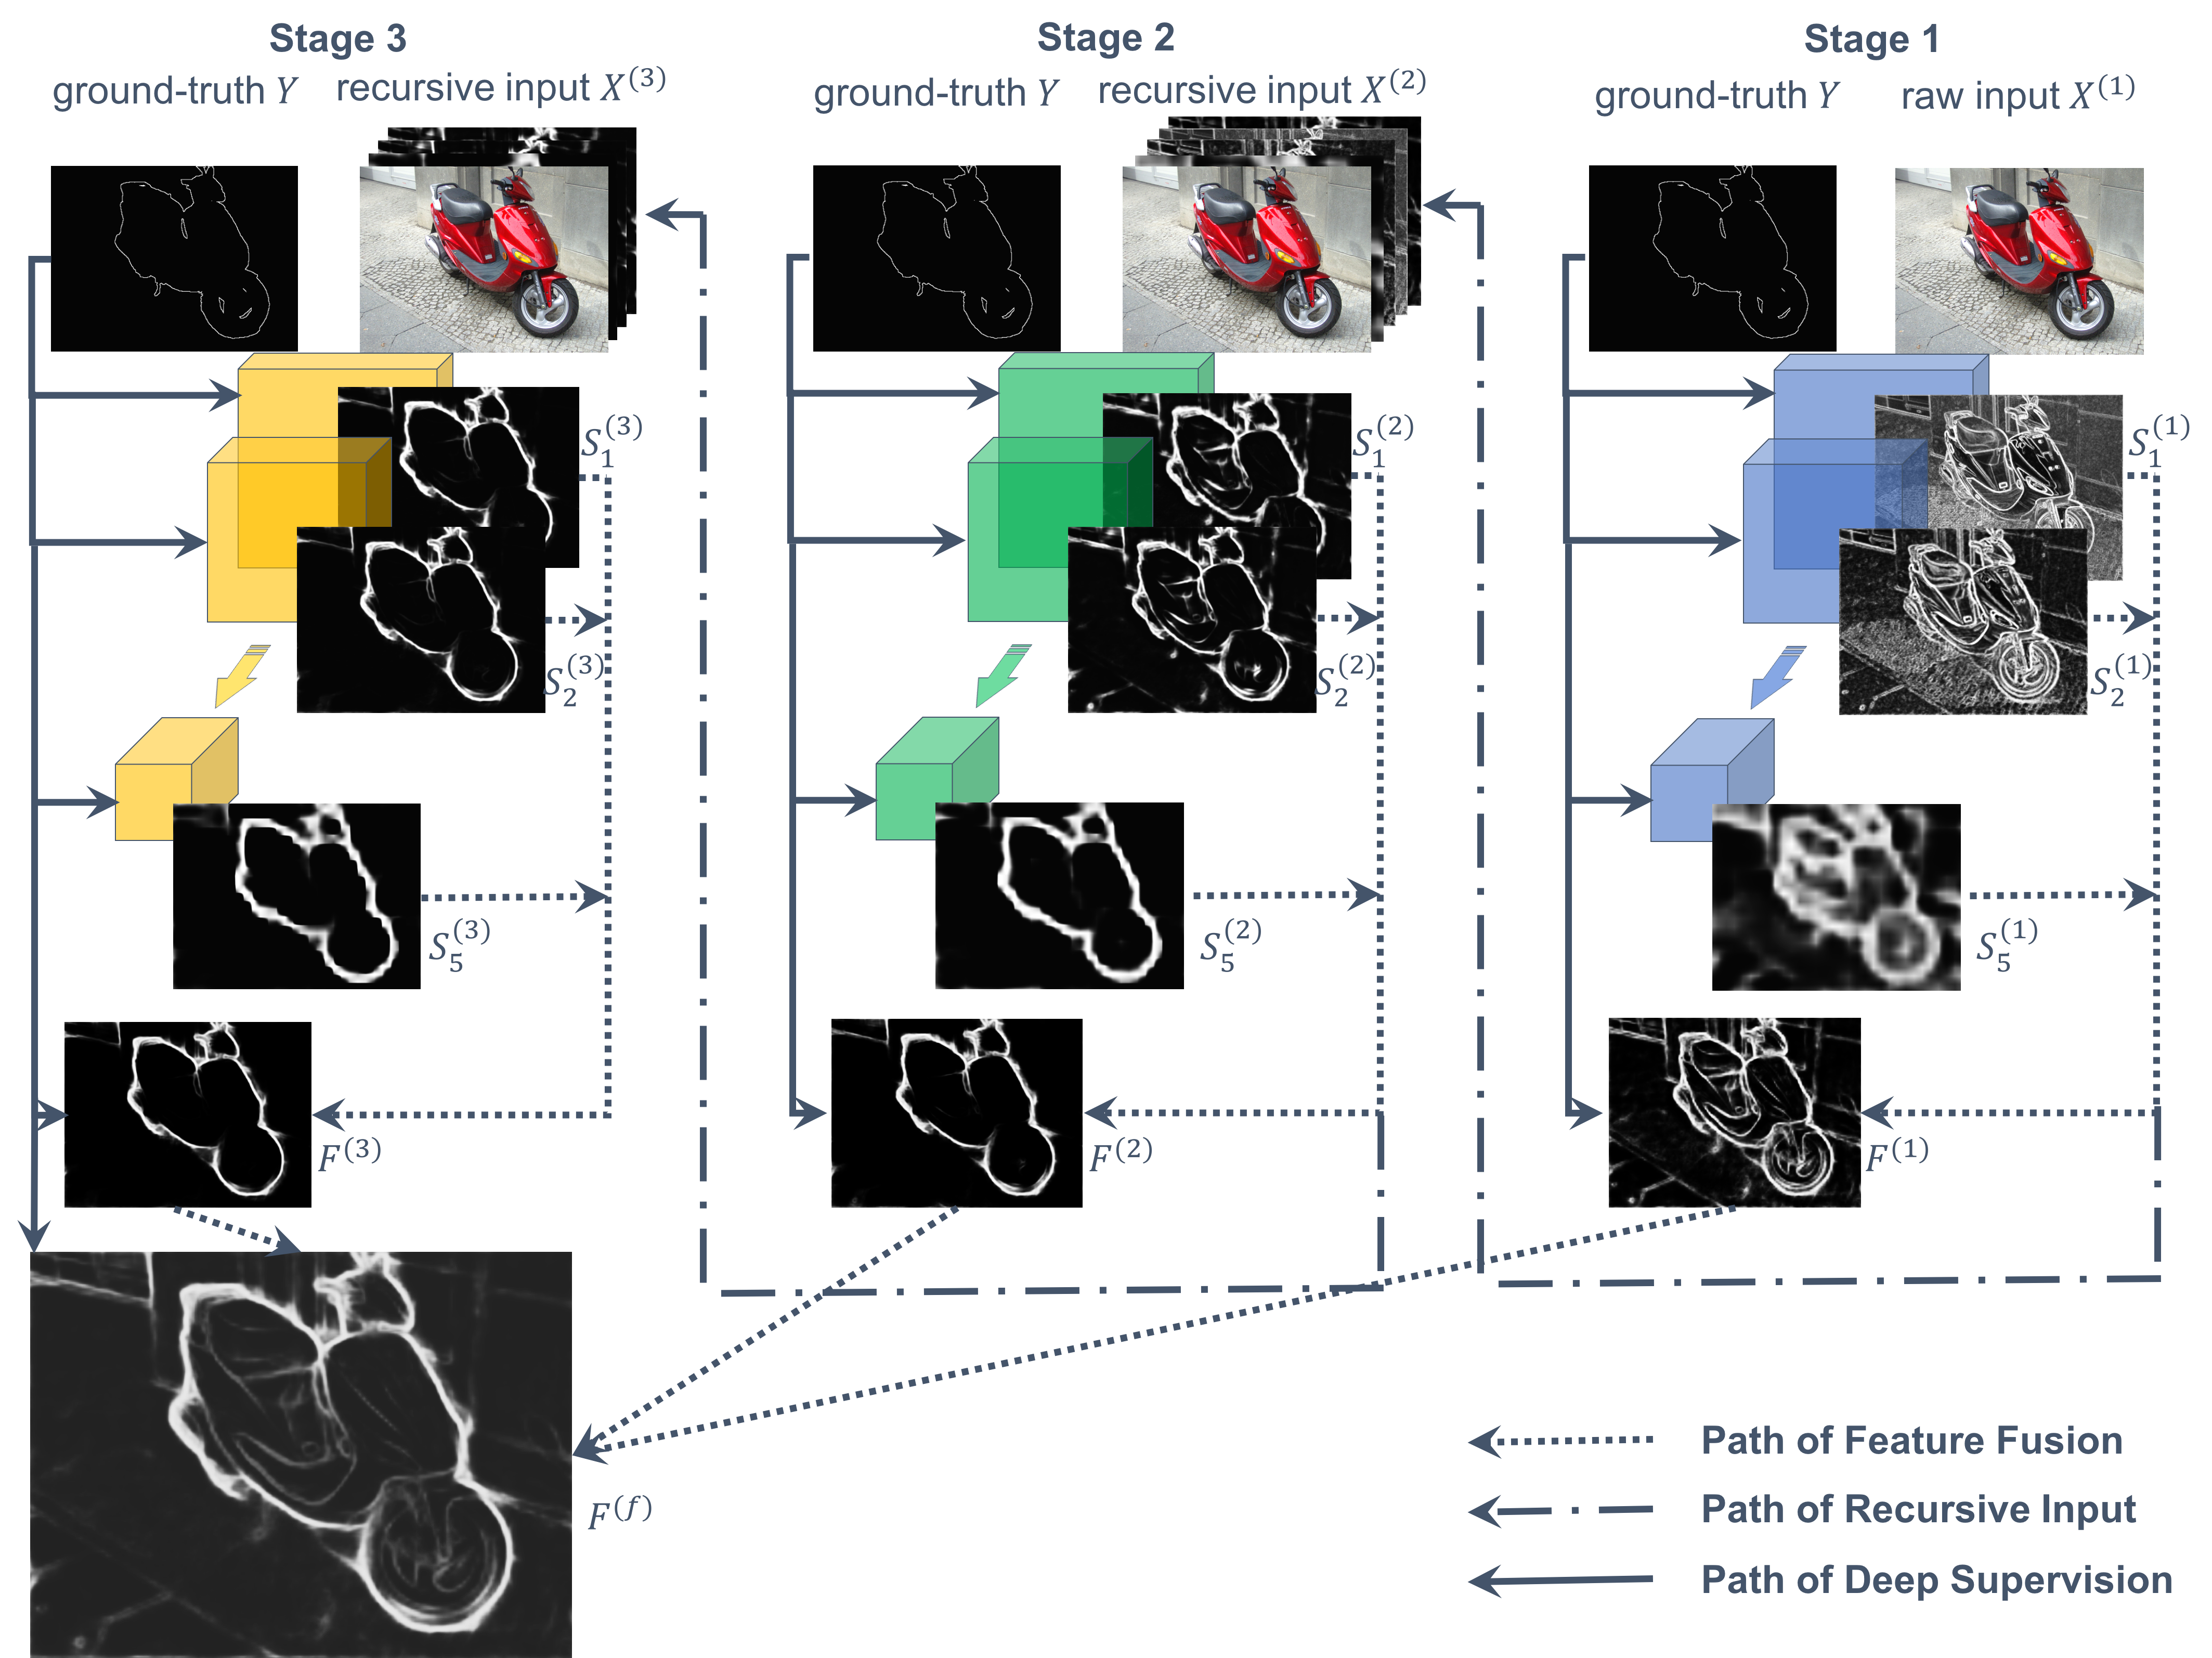
\includegraphics[width=15cm]{network.png}\\
  \caption{Illustration of the proposed cascaded fully convolutional network for object boundary detection.}\label{network}
\end{figure}


\section{Training Phase} \label{training phase}

Object Boundary Detection can be formulated as a pixel-wise two-class classification problem. Given a training image \(X = (X(j), j = 1, 2, ..., |X|)\) with totally |X| pixels over the spatial dimensions, our goal is to classify each \(\tilde{Y}(j)\), the label of pixel \(X(j)\), as a boundary pixel (\(\tilde{Y}(j) = 1\)) or not (\(\tilde{Y}(j) = 0\)). And we use \(\tilde{Y} = (\tilde{Y}(j), j = 1, 2, ..., |X|)\) to denote the corresponding detected boundary map. Considering the mini-batch with size equal to \(Z\), and the network with \(P\) sub-networks and \(Q\) levels in each sub-network, we demonstrate our end-to-end training as follows.

\subsection{Formulation of the Multi-recursive-input}
Let \(S_{p}^{(q)}\) be the side-output of the \(p^{th}\) level in the \(q^{th}\) sub-network, \(F^{(q)}\) and \(X^{(q)}\) be the fused prediction and training input in the \(q^{th}\) sub-network, now we have:

\begin{eqnarray}
X^{(q)} &=& 
\begin{cases} 
X &, q = 1 \cr
X \circ S_{q-1}^{1} \circ S_{q-1}^{2} \circ \cdots \circ S_{q-1}^{Q} &, q > 1 \cr
\end{cases}
\end{eqnarray}
Here \(\circ\) represents the concatenating operation along with the color channel. 

\subsection{Loss Function}
To demonstrate the loss function of our cascaded network, we firstly present the loss function of side-output \(S_{p}^{(q)}\):

\begin{eqnarray}
\begin{split}
l_{p}^{(q)}(\textbf{W}^{(q)}, \textbf{w}_{p}^{(q)}; X^{(q)}, Y)
=&-\alpha \sum_{j\in{|B|}}log(1 - sigmoid(s_{p}^{(q)}(j))) \\
&-(1-\alpha) \sum_{j\in{|\bar{B}|}}log(sigmoid(s_{p}^{(q)}(j)))
\end{split}
\end{eqnarray}

where \(\textbf{W}^{(q)}\), \(\textbf{w}_{p}^{(q)}\), \(|B|\) and \(|\bar{B}|\) refer to the model parameters of the \(q^{th}\) sub-network, ones of the \(S_{p}^{(q)}\), the sets of boundary and non-boundary ground-truth annotations, respectively. \(\alpha\) is the ratio of \(|\bar{B}|\) and \(|B|\), which cancels out the huge imbalance of positive samples (boundary pixels) and negative samples (non-boundary pixels) in some degree\cite{Xie2015}. 

Let \(\beta_{p}^{(q)}\) be the weight of \(S_{p}^{(q)}\). Given the notation as follows:

\begin{eqnarray*}
\textbf{W} &=& \{\textbf{W}_{1}, \textbf{W}_{2}, \cdots , \textbf{W}^{(q)}\}, \\
\textbf{w} &=& (\textbf{w}_{p}^{(q)}, p from 1 to P and q from 1 to Q), \\
\end{eqnarray*}
the loss of all the side-outputs in the \(q^{th}\) sub-network, \(L_S\), is the sum of the losses of all its side-outputs and the fusion output.

\begin{eqnarray}
L_S(\textbf{W}, \textbf{w}; X, Y) &=& \sum_{q=1}^{Q}\sum_{p=1}^{P}\beta_{p}^{(q)}l_{p}^{(q)}(\textbf{W}^{(q)}, \textbf{w}_{p}^{(q)}; X^{(q)}, Y)
\end{eqnarray}

All the side-outputs in one stage are fused through a 1 \(\times\) 1 convolution layer as mentioned in Section \ref{network structure}. The fusion of \(q^{th}\) sub-network is defined as:

\begin{eqnarray} \label{fusion of subnet}
F^{(q)} &=& \sum_{p=1}^{P}\theta_{p}^{(q)}S_{p}^{(q)}
\end{eqnarray}
where \(\theta_{p}^{(q)}\) is the fusion weight of \(S_{p}^{(q)}\).

The fusion loss of \(q^{th}\) stage is:

\begin{eqnarray}
\begin{split}
l_{f}^{(q)}(\textbf{W}^{(q)}, \textbf{w}^{(q)}; X^{(q)}, Y)
=&-\alpha \sum_{j\in{|B|}}log(1 - sigmoid(F^{(q)}(j))) \\
&-(1-\alpha) \sum_{j\in{|\bar{B}|}}log(sigmoid(F^{(q)}(j)))
\end{split}
\end{eqnarray}
where \(\textbf{w}^{(q)}\) is the set of the parameters for all the side-outputs in stage \(q\).

Similar to Function \ref{fusion of subnet}, the final prediction is produced by:

\begin{eqnarray}
F^{(f)} &=& \sum_{q=1}^{Q}\phi^{(q)}F^{(q)}
\end{eqnarray}
where \(\phi^{(q)}\) is the fusion weight of \(F^{(q)}\).

The loss of all the fusion outputs is:
\begin{eqnarray}
L_{f}(\textbf{W}, \textbf{w}, \mathbf{\theta}, \mathbf{\phi}; X, Y) &=& \sum_{q=1}^{Q}\beta_{f}^{(q)}l_{f}^{(q)}(\textbf{W}^{(q)}, \textbf{w}^{(q)}; X^{(q)}, Y)
\end{eqnarray}
where \(\mathbf{\theta} = (\theta_{p}^{(q)}, q = 1, 2, ... , Q, p = 1, 2, ... , P)\), \(\mathbf{\phi} = (\phi^{(q)}, q = 1, 2, ... , Q)\) and \(\beta_{f}^{(q)}\) denotes the loss weight for each sub-network.

Finally, we train all the parameters jointly in an end-to-end framework by minimize the following total loss:
\begin{eqnarray}
L_{t}(\textbf{W}, \textbf{w}, \mathbf{\theta}, \mathbf{\phi}; X, Y) &=& L_S(\textbf{W}, \textbf{w}; X, Y) + L_{f}(\textbf{W}, \textbf{w}, \mathbf{\theta}, \mathbf{\phi}; X, Y)
\end{eqnarray}

\section{Testing Phase} \label{testing phase}
When testing, we input an image \(X\) into the first sub-network and obtain the fusion of each sub-network as Function \ref{fusion of subnet}, step by step. Considering the \(q^{th}\) stage as a function \(f^{(q)}\), the final prediction \(\tilde{Y}\) can be produced by:

\begin{eqnarray}
\tilde{S}_{p}^{(q)} &=& f^{(q)}(X^{(q)}, (\textbf{W}^{(1)})^{*}, ... , (\textbf{W}^{(Q)})^{*}, (\textbf{w}_{1}^{(Q)})^{*}, ... , (\textbf{w}_{P}^{(Q)})^{*}) \\
\tilde{F}^{(q)} &=& \sum_{p=1}^{P}(\theta_{p}^{(q)})^{*}\tilde{S}_{p}^{(q)} \\
\tilde{F}^{(f)} &=& \sum_{q=1}^{Q}(\phi^{(q)})^{*}\tilde{F}^{(q)} \\
\tilde{Y} &=& sigmoid(\tilde{F}^{(f)})
\end{eqnarray}

\begin{figure}[t]
  \centering
  % Requires \usepackage{graphicx}
  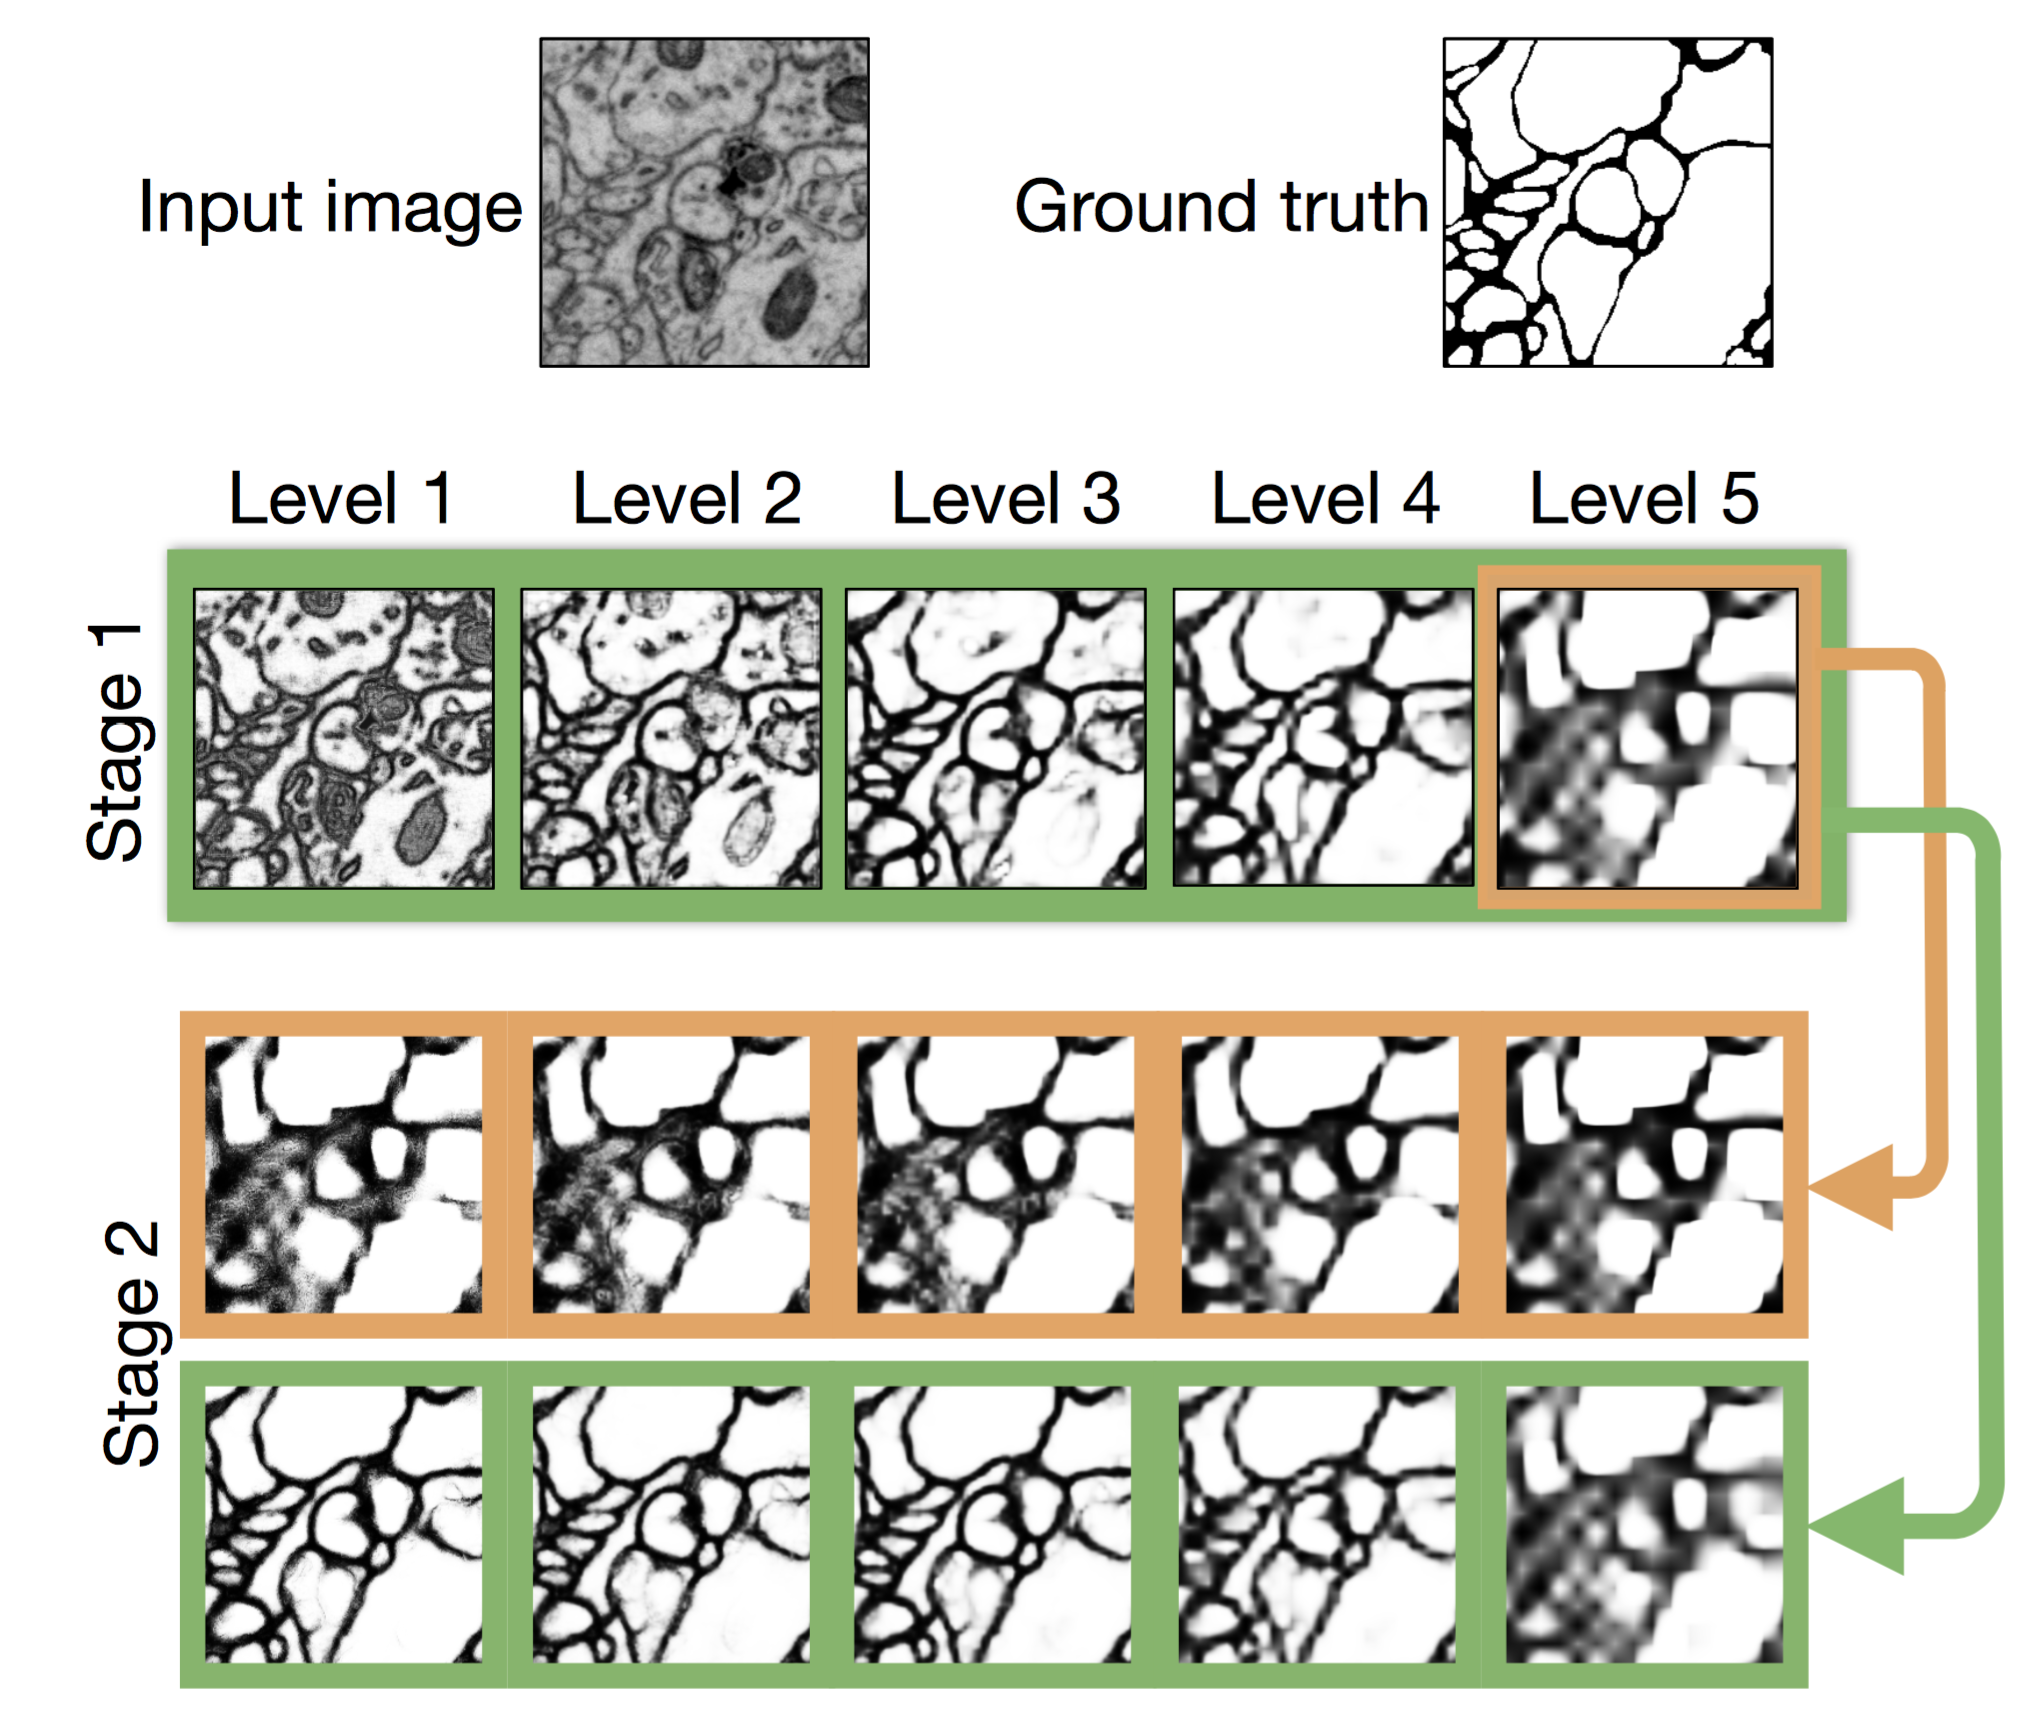
\includegraphics[width=15cm]{multi-recursive-input.png}\\
  \caption{Multi-recursive-input \emph{vs.} Single-recursive-input.}\label{multi recursive input}
\end{figure}

\section{Model Interpretation} \label{interpretation}
\subsection{Cascaded Architecture \emph{vs.} Single-stage Architecture}
Such a cascaded architecture for object-level boundary detection can be interpreted as follows:

On one hand, our eyes can capture various levels of data due to the information re-organization achieved by the multi-stage vision system in our brain.The proposed cascaded architecture mimics the multi-stage vision system of human-beings, by introducing the recursive links to re-filter the multi-scale features produced by the previous stage. As illustrated in Fig. \ref{interpretation_png}, to compare the side-outputs and fusions in row (in the same level), we find the boundary map of each stage is \emph{"clearer"} than the former stage. The cascaded network enables the later layers to have a higher-level scope, which breaks the limitation of the receptive filed size existing in a single-stage network. Comparing with a considerably deep single-stage network which has the same receptive size, in other words, our cascaded network will not suffer from the gradient vanishing  and be much easier to be trained.

On the other hand, human can see both the local details and the object-level abstracts from an image, while not confused by the complex multi-scale information. It is mainly because our brain has a multi-stage vision system to filter these information and select the useful information from the right scale\cite{Helmstaedter2013}. the joint training and feature fusion of the proposed method let data drives the choice from the results of all the stages and levels.

\subsection{Multi-recursive-input \emph{vs.} Single-recursive-input}

One of the biggest differences between our work with others is the multi-recursive-input. The qualitative comparison can be found in Fig. \ref{multi recursive input}, where the single-recursive-input only reuses the large scale features in the next stage and thus loses the ability to accurately localize the boundary.

\begin{figure}[t]
  \centering
  % Requires \usepackage{graphicx}
  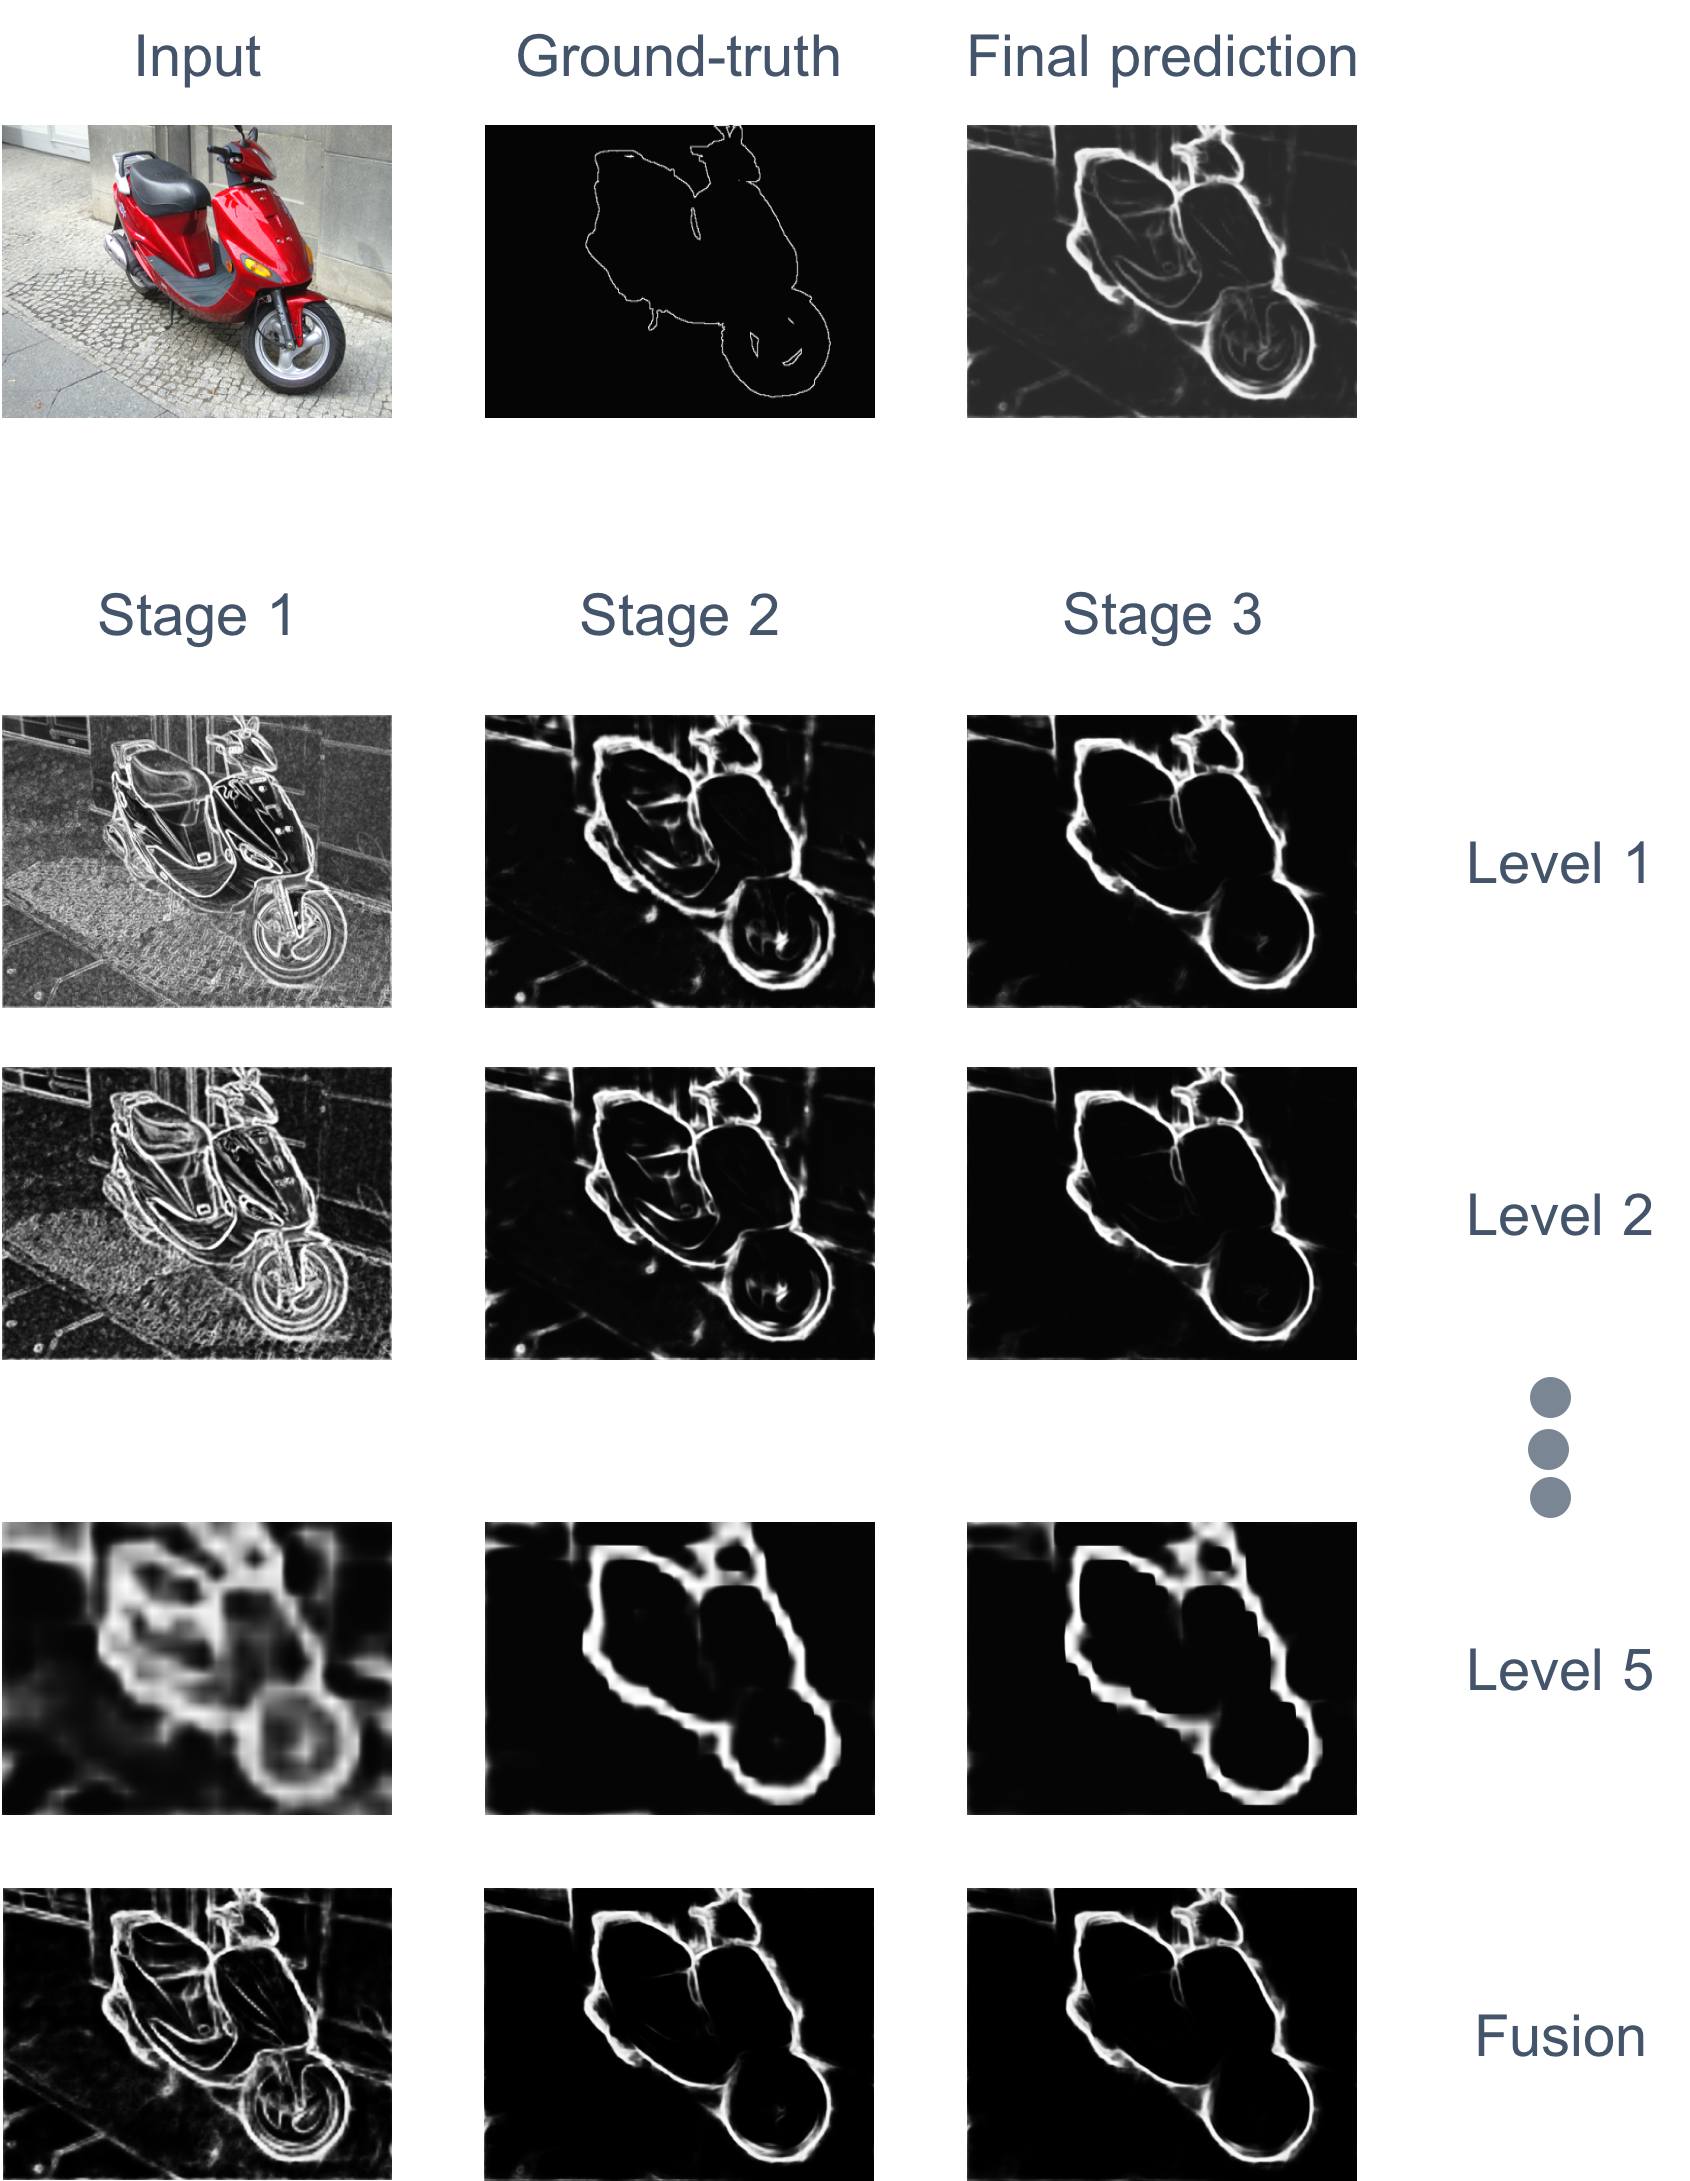
\includegraphics[width=15cm]{interpretation.png}\\
  \caption{Prediction exmaples from different side-outputs and fused outputs in different stages.}\label{interpretation_png}
\end{figure}

\subsection{End-to-end Training \emph{vs.} Stepwise Self-tuning}
To train our network end-to-end, the former stages and the next stages can have an effect on each other. Instead of fixing the model parameters of the previous stages, we let data teach how the network works. With enough training data and the proposed easy-to-train network architecture, our network is able to adjust all the parameters jointly and benefit from it to achieve a better performance than trained stepwise. Refer to Chapter \ref{experiments} for quantization results and details.

%%%%%%%%%%%%%%%%%%%%%%%%%%%%%%%%%%%%%%%%%%%%%%%%%%%%%%%%%%%%%%%%%%%%%%%%%%%%%%%


\chapter{Experiments} \label{experiments}
As addressed in Chapter \ref{introduction}, we firstly test our cascaded fully convolutional network in the task of neuronal boundary detection on two mainstream datasets, Mouse Piriform Cortex Dataset\cite{Lee2015} and ISBI 2012 EM Segmentation Dataset\cite{Ronneberger2015}, then extend to adapt with the object boundary detection in natural images on the large object boundary dataset, PASCAL VOC Contour Dataset\cite{Yang2016}. Besides, we will give the comparative experiments to explain how the performance is achieved by the proposed network structure.

\section{Neuronal Boundary Detection in EM Images}

Neuronal boundary detection in EM images is usually formed as the segmentation annotation problem (Fig. \ref{segmentation and boundary}). In training phase, we compute the 2D gradient in the segmentation ground-truth to obtain the boundary annotation. And then in testing phase, we apply the graph-based algorithms such as watershed algorithm to transfer the boundary prediction into segmentation, since the evaluation metric is based on the segmentation results. In this experiment, we firstly detect the membrane boundary and then apply graph-based watershed\cite{Zlateski2015} to it for a segmentation result.

\subsection{Evaluation Metric}

We follow the metric proposed in \cite{Lee2015}, using the Rand F-score to report the performance of the segmentation. As the harmonic average of the Rand merge score and Rand split score, marked as \(V_{merge}^Rand\) and \(V_{split}^Rand\) respectively, the Rand F-score:

\begin{eqnarray}
V_{Fscore}^{Rand} = \frac{2 V_{merge}^{Rand} V_{split}^{Rand}}{V_{merge}^{Rand} + V_{split}^{Rand}}\\
\end{eqnarray}
and 
\begin{eqnarray}
V_{merge}^{Rand} = \frac{\sum_{ij} p(i, j)^2}{\sum_i(\sum_j p(i, j))^2} \\
V_{split}^{Rand} = \frac{\sum_{ij} p(i, j)^2}{\sum_j(\sum_i p(i, j))^2}
\end{eqnarray}
where \(p(i, j)\) indicates the number of pixel pairs located in the \(i^{th}\) segment of the detected segmentation and the \(j^{th}\) segment of the ground-truth segmentation.

Rand split score is high for those results with few split errors, while Rand merge score is high for those results with few merge errors. Generally there will be a trade-off between the Rand split score and the Rand merge score for an image or a dataset. The Rand F-score here is to define the trade-off score, just like the role of the F-score or F-measure in many object detection benchmarks to average the precision metric and recall metric.

The Precision (rand merge)-recall (rand split) curves \emph(PR-curves) can be generated by varying the threshold for boundary binarization\cite{Shen2016CVPR}.

\begin{figure}[t]
  \centering
  % Requires \usepackage{graphicx}
  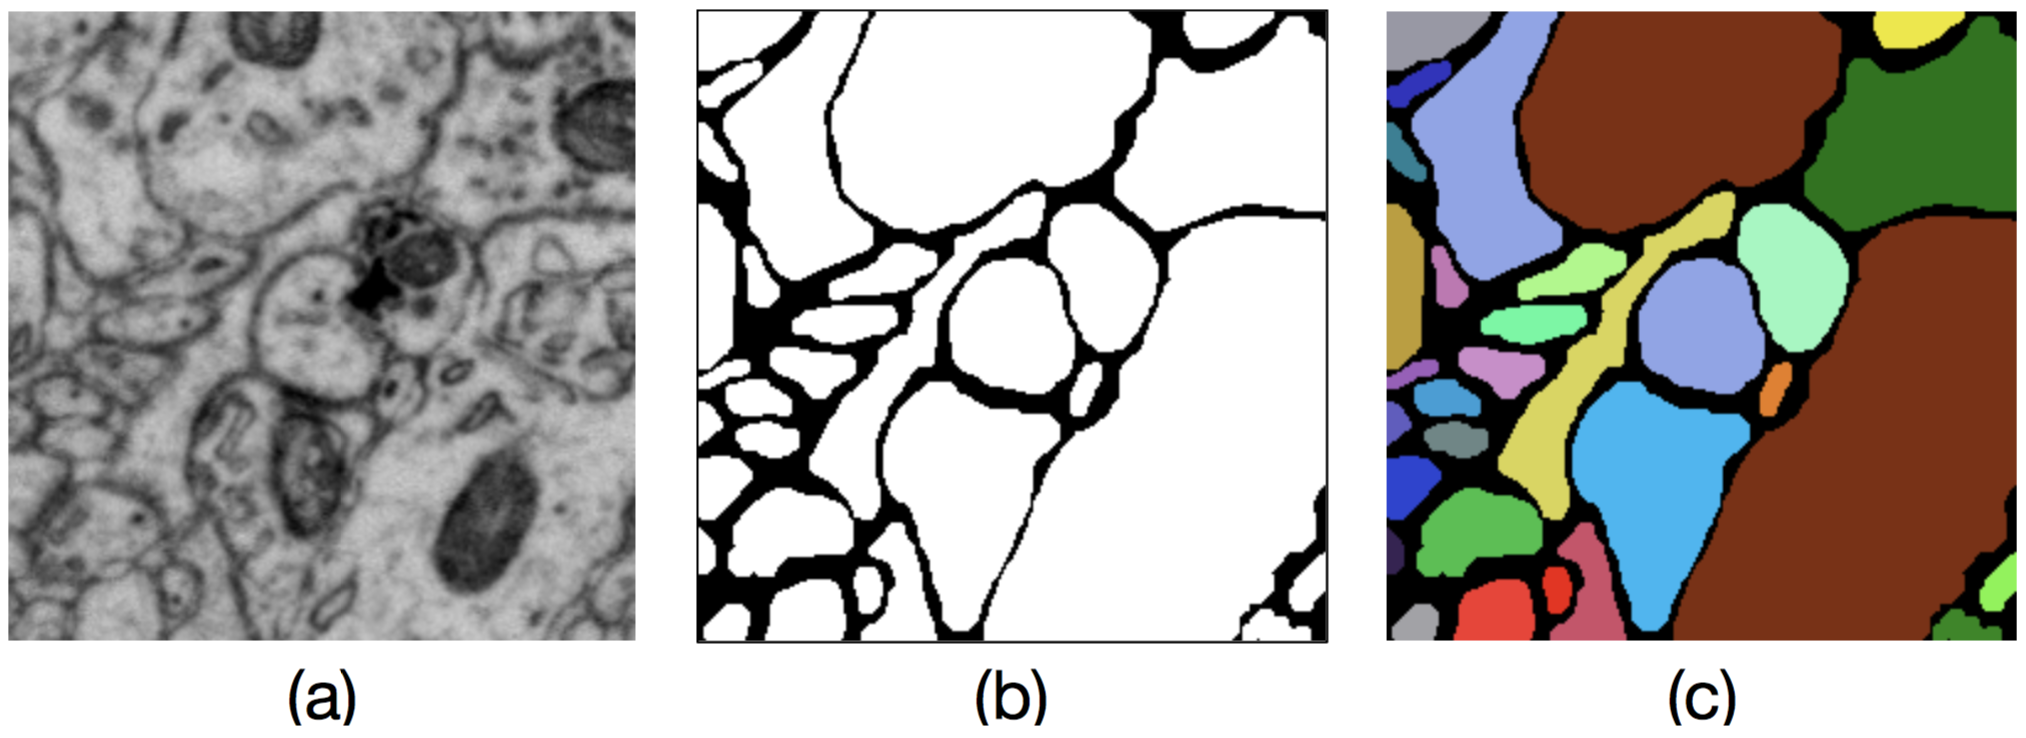
\includegraphics[width=15cm]{segmentation_and_boundary.png}\\
  \caption{(b)Neuronal boundary detection and (c) segmentation can be easily converted from each other, which we used in the experiments on Mouse Piriform Cortex Dataset\cite{Lee2015} and ISBI 2012 EM Segmentation Dataset\cite{Ronneberger2015}. (1) By applying the graph-based algorithms such as watershed, we can transfer the boundary prediction into segmentation. (2) By calculating the 2D gradient in the segmentation ground-truth, the boundary annotation can be obtained. }\label{segmentation and boundary}
\end{figure}

\subsection{Mouse Piriform Cortex Dataset}\label{experiment of piriform}

Mouse Piriform Cortex Dataset\cite{Lee2015} contains 4 stacks of grayscale EM images and their corresponding segmentation annotations(Table. \ref{piriform_dataset}), where the stack 1 for validation and the stack 2, 3, 4 for training. 

\begin{table}[t]
\renewcommand{\arraystretch}{1.2}
\caption{Mouse Piriform Cortex Dataset}
\label{piriform_dataset}
\begin{center}
\begin{tabular}{|c|c|c|c|c|c|c|c|}
\hline
\multicolumn{1}{|c|}{}
&\multicolumn{1}{c|}{stack 1}
&\multicolumn{1}{c|}{stack 2}
&\multicolumn{1}{c|}{stack 3}
&\multicolumn{1}{c|}{stack 4}
\\
\hline
Slices	&	168	&	170		&	169		&	121		\\	\hline
Scales	&	255*255	&	512*512		&	512*512		&	256*256		\\	\hline
Usage	&	Validation	&	Training		&	Training		&	Training		\\	\hline
\end{tabular}
\end{center}
\end{table}

The annotation of EM images is laborious and time consuming\cite{Helmstaedter2013}, leading to the lack of annotated training samples in EM boundary detection. However, the deep networks often require thousands of training data to drive the optimization algorithms. So we augment the raw data to generate sufficient data for training, by rotating the raw image into four directions \((0, \frac{\pi}{2}, \pi, \frac{3\pi}{2})\), then flipping them with three cases (horizontal flipping, vertical flipping, no flipping), and rescaling them to three scales \((0.8, 1.0, 1.2)\), resulting in the training data 36 times the raw images.

To train such a considerably large network from scratch is not necessary nor effective, so we follow the framework proposed by a lot of works\cite{Long2015, Xie2015, Shen2016CVPR} to initialize model parameters of the first stage with the VGG-16 models pre-trained in ImageNet\cite{Deng2009}. To ease the multi-stage training, we train a single-stage model first. Then use it to initialize the first stage of a two-stage network, leaving the second stage is initialized randomly, by which our multi-stage networks can reuse the relatively low-level filters learned by the single-stage network. Note that the proposed cascaded network is still trained end-to-end because we do not fix any parameters in the final training step but train all the parameters jointly instead. 

For experiment settings, we use the standard SGD algorithm to optimize the network, with the momentum of 0.9, the weight decay of 2 \(\times\) \(10^{-4}\), and a stepwise learning rate from 1e-8 to 1e-9(after 20000 iterations). By default, there are 5 convolution levels in each subnet. The training for the takes 20000 iterations for the single-stage network, and 10000 iterations for each of the sequential sub-networks. 

Quantitative results are shown in Table \ref{piriform fscore} and Fig. \ref{piriform prcurve}. With stacking the sub-networks, our method can maintain both a high recall and a high precision. Compared with the current state-of-the-art method VD2D3D\cite{Lee2015}, a deep network with the parameters of several layers fine-tuned by recursively input the prediction into itself, our 2-stage and 3-stage cascaded network can outperform it by around 1\% and 1.5\% respectively. We argue that such a improvement is meaningful in neuronal boundary detection, since the precise boundary annotation is vital for neural circuits reconstruction and has a low tolerance of errors.The architecture of VD2D3D is much like the Fig. \ref{cascade_structures}(c), while the VD2D3D not only feeds the boundary map of the raw input but also generates the predictions of neighbor slices and concatenates all them to enhance the learning (Fig. \ref{Lee2015}). Our networks, taking advantage of the multi-recursive-input and end-to-end training, can outperform the VD2D3D without any additional 3D context information. 

\begin{table}[t]
\renewcommand{\arraystretch}{1.2}
\caption{Rand F-scores on Mouse Piriform Cortex Dataset\cite{Lee2015}}
\label{outcome}
\begin{center}
\begin{tabular}{|c|c|c|c|c|}
\hline
&\multicolumn{1}{c|}{Rand Split Score}
&\multicolumn{1}{c|}{Rand Merge Score}
&\multicolumn{1}{c|}{Rand F-score}\\
\hline
N4\cite{Ciresan2012} 			& 0.9010 	& 0.9619 	& 0.9304	\\	\hline
VD2D\cite{Lee2015} 		& 0.9174	& 0.9771 	& 0.9463 	\\	\hline
VD2D3D\cite{Lee2015}	& 0.9555	& 0.9891	& 0.9720    \\	\hline
Ours(1-stage) 			& 0.9802 	& 0.9576	& 0.9688	\\	\hline
Ours(2-stage) 			& \textbf{0.9880}	& 0.9759 	& 0.9819 	\\	\hline
\textbf{Ours(3-stage)} 	& 0.9815 	& \textbf{0.9917} 	& \textbf{0.9866} 	\\	\hline
\end{tabular}
\end{center}
\label{piriform fscore}
\end{table}

\begin{figure}[t]
  \centering
  % Requires \usepackage{graphicx}
  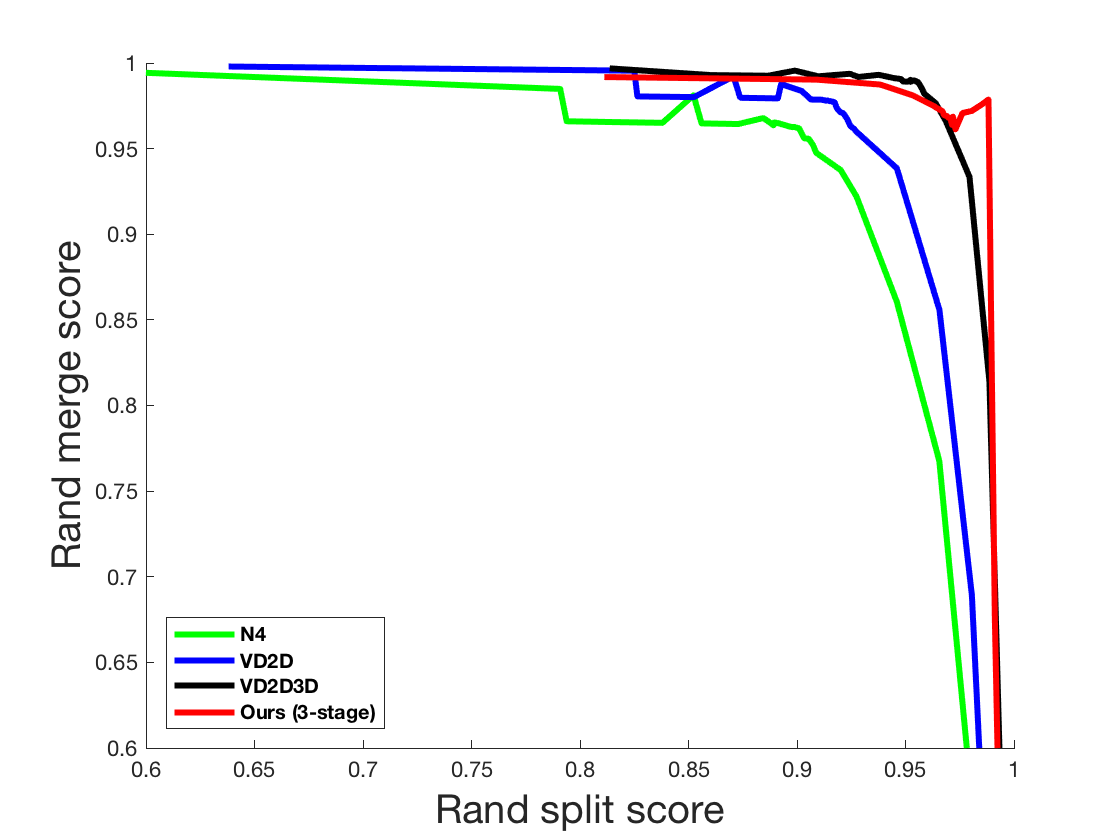
\includegraphics[width=15cm]{piriform prcurve.png}\\
  \caption{Precision (rand merge)-recall (rand split) curves on Mouse Piriform Cortex Dataset\cite{Lee2015}. Our 3-stage network outperforms all the previous works on this dataset.}\label{piriform prcurve}
\end{figure}

\subsection{ISBI 2012 EM Segmentation Dataset}
The other dataset for neuronal boundary detection in EM images is the ISBI 2012 EM Segmentation Dataset. As the dataset for the popular ISBI 2012 EM Segmentation Challenge, ISBI 2012 EM Segmentation Dataset does not offer the ground-truth segmentation for the testing stack, which is reasonable but increases the difficulty of results analyzing and discussion. Besides, the raw training data with annotations are relatively insufficient, where there is only one stack for training with the dimension of 30 \(\times\) 512 \(\times\) 512. To train a very deep network using such a few images is theoretically difficult, even though we use the standard data augmentation to enrich the training materials. 

Network settings are the same as ones we used in the experiment for Mouse Piriform Cortex Dataset\cite{Lee2015}. Standard data augmentation (Section \ref{experiment of piriform}) is considered here, too.

The Rand F-score data from the leaderboard of ISBI 2012 EM Segmentation Challenge are shown in Table \ref{isbi12 fscore} . Not all the scores are presented since there are many entries in the leaderboard which have not been reported in literature. It worths noting that most of the leading methods apply post-processing algorithms or assemble several models to improve the ranking. However, the proposed cascaded networks without any post-processing procedures can achieve competitive result to those with post-processing. 
The post-processing used in each approach is also presented in Table \ref{isbi12 fscore}, where \cite{Beier2016} is a post-processing algorithm itself and can be adopted to ours. With a proper post-processing, our network can win the state-of-the-art with more powerful ResNet\cite{He2016} as its base network. In the future, we will embed the ResNet\cite{He2016} in our cascaded framework to further improve the performance.


\begin{table}[t]
\renewcommand{\arraystretch}{0.8}
\caption{The Rand F-scores part from the leaderboard of ISBI 2012 EM Segmentation Challenge\cite{Ronneberger2015}.}
\label{outcome}
\begin{center}
\begin{tabular}{|c|c|}
\hline
&\multicolumn{1}{c|}{Rand F-score}\\
\hline
U-net\cite{Ronneberger2015} 			& 0.9727	\\	\hline
CUMedVision\cite{Chen2016} 			& 0.9768 	\\	\hline
IAL IC\cite{Beier2016}			& 0.9773	 \\	\hline
FusionNet\cite{Quan2016} 			& 0.9780	\\	\hline
Ours(3-stage) 			& 0.9780	\\	\hline
PolyMtl\cite{Drozdzal2017} 			& 0.9806	\\	\hline
Ours(3-stage) + IAL IC			& 0.9836	\\	\hline
\end{tabular}
\end{center}
\label{isbi12 fscore}
\end{table}



\section{Object Boundary Detection in Natural Images}

\begin{figure}[t]
  \centering
  % Requires \usepackage{graphicx}
  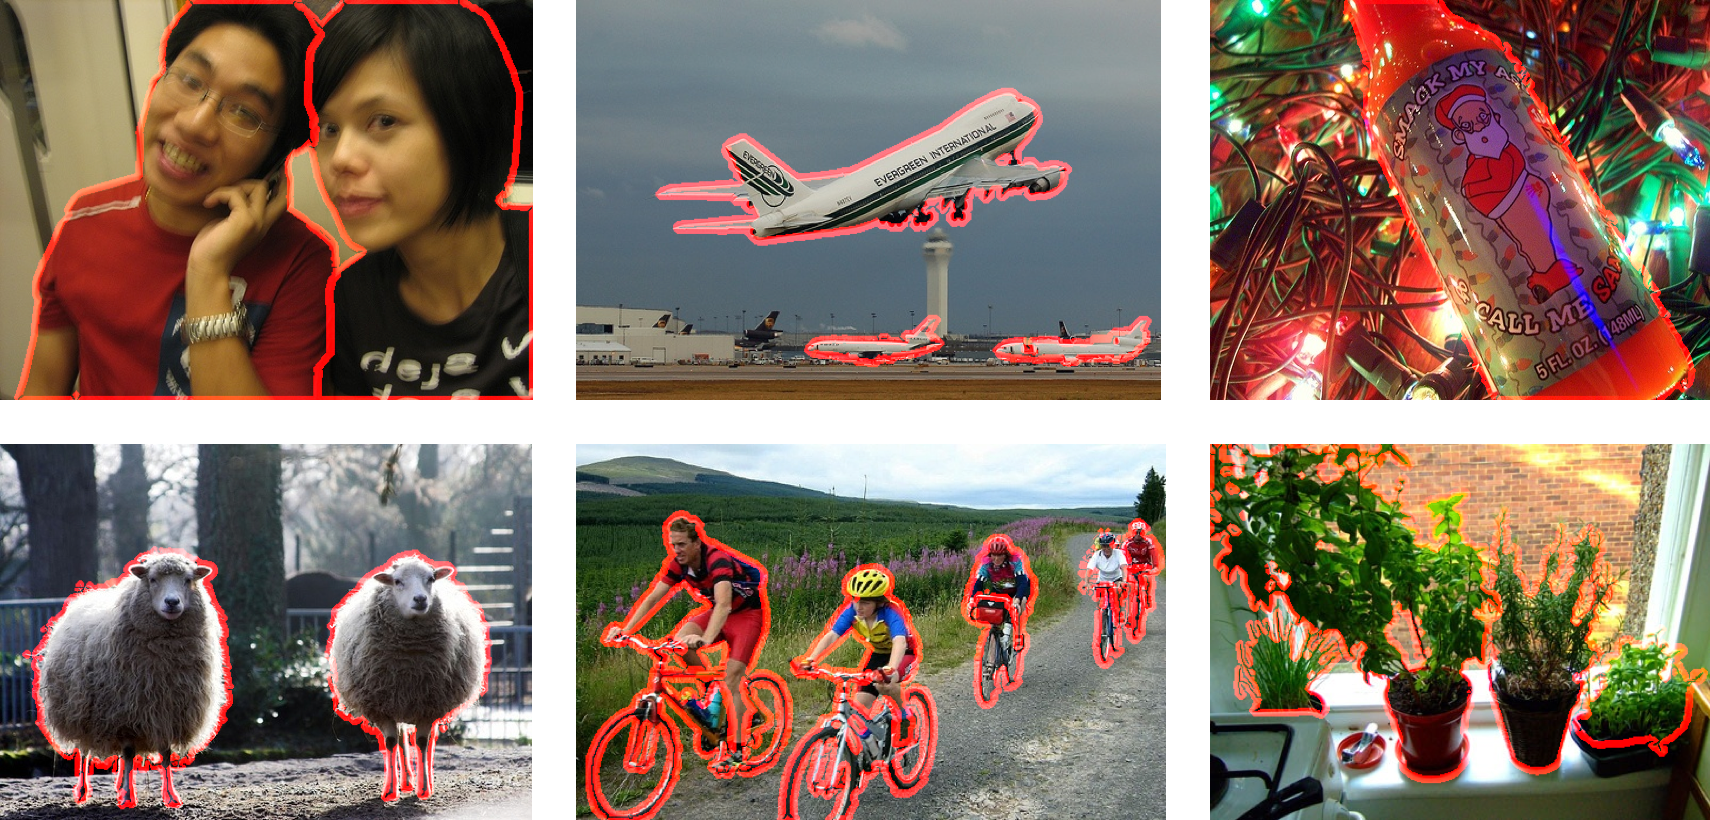
\includegraphics[width=15cm]{voc_contour.png}\\
  \caption{Examples selected from PASCAL VOC Contour Dataset\cite{Yang2016}, where ground-truth contours are labeled as red. There are various objects (human, artificialities, animals, plants, etc.) appearing in complex scenes (indoor and outdoor environments, colorful backgrounds, blurs, textural confusions, etc), which significantly increases the difficulty of detecting the object-level boundary.}\label{voc contour}
\end{figure}

Our work begins at Neuronal Boundary Detection of EM images but dose not end in it. By applying the proposed multi-stage network to common object boundary detection in natural images, we evaluate the generalization capacity of our network.

\subsection{Metrics}
Precision and Recall are the well-accepted metrics for two-class annotation tasks\cite{Shen2016CVPR, Shen2017TIP, Yang2016}. Given the notations as follows: 
(1) True Positive \emph{(TP)}: the times of annotating a positive pixel as positive;
(2) False Positive \emph{(FP)}: the times of annotating a negative pixel as positive;
(3) True negative \emph{(TN)}: the times of annotating a negative pixel as negative;
(4) False positive \emph{(FN)}: the times of annotating a positive pixel as negative;
we have Precision \emph{(P)}, Recall \emph{(R)} and their harmonic average F-measure

\begin{eqnarray}
P &=& \frac{TP}{TP+FP} \\
R &=& \frac{TP}{TP+FN} \\
F-measure &=& \frac{2PR}{P+R} \\
\end{eqnarray}

The Precision-Recall Curve \emph(PR-curves) can be also generated by varying the threshold for boundary binarization\cite{Shen2016CVPR}.

\subsection{PASCAL VOC Contour Dataset}
PASCAL VOC Segmentation Datasets are a series of well-accepted object segmentation datasets,  including the well-annotated natural photos released from 2007 to 2012. \cite{Yang2016} apply DenseCRF\cite{Krahenbuhl2011} to further refine the boundary annotation from the segmentation ground-truth and release a large instance-level object boundary detection dataset, PASCAL VOC Contour Dataset, with 10582 training images, 1449 testing images and their corresponding boundary annotations. Different from EM images, these natural photos are taken from various scenes and contain kinds of objects (Fig. \ref{voc contour}). For example, in each photo, the image scale, the number and category of the object are different. There are also many samples with blurred object boundary and confused background on the dataset. All these significantly increase the difficulty of boundary detection on the PASCAL VOC Contour Dataset, while call out a deep network with sufficient capacity to extract the highly abstract object-level features from the data.

With such a large dataset, the standard data augmentation with a ratio of 36 is not necessary nor efficient. We follow the light-weight data augmentation mentioned in \cite{Yang2016}, by randomly cropping four 224 \(\times\) 224 patches from the raw image and flipping them once, resulting in 8\(\times\) training samples. Here, the cropping is mainly for memory efficiency\cite{Yang2016} and the mini-batch based training. Original FCNs\cite{Long2015} is not available for the training with multiple training samples in one mini-batch, because these samples may have different scales and can result in error. By fixing the cropped patches into one-size, we are able to enlarge the batch-size, 8 in practice, for a more effective and faster training.

We fine-tune the proposed network on PASCAL VOC Contour Dataset using the same strategy in Section \ref{experiment of piriform}. Firstly, we train a single-stage network with the same structure as HED\cite{Xie2015}. Then we use the fine-tuned HED network to initialize the training for our 2-stage and 3-stage cascaded fully convolutional networks. F-measure comparisons are shown in \ref{voc fscore}. 

For optimization, we use the standard Stochastic Gradient Descent \emph{(SGD)}. Other hyper parameters such as the level of convolution in each subnet, learning rate, momentum and weight decay are same as what we used in the experiments of neuronal boundary detection. As demonstrated in \cite{Yang2016}, to process all the training samples, named one epoch, takes around 10000 iterations. We train the single-stage, 2-stage and 3-stage networks for 2 epochs, 4 epochs, and 5 epochs respectively. Compared with the CEDN proposed in \cite{Yang2016}, the training for our cascaded networks costs only half of the time for training CEDN, which proves the effectiveness of the proposed recursively end-to-end training.

As we expected, traditional methods for local edge detection such as SCG, its multi-scale version MCG\cite{Arbelaez2014}, and Structured Random Forest for Edge Detection \emph{(SE)}\cite{Dollar2013} present poor results on this benchmark. These methods use hand-crafted features which often combine multiple cues like color, brightness, spectrum, to handle different cases. HED\cite{Xie2015} has the ability to naturally obtain the hierarchical features due to the adoption of the holistically-nested network, which is also used in our sub-networks. We fine-tune it on PASCAL VOC Contour Dataset and receive a F-measure of 0.52, much better than the traditional methods but lower than our 2-stage network. What's more, our 3-stage network outperforms CEDN\cite{Yang2016} by 2\% and achieves the state-of-the-art score on this benchmark. PR-curves in Fig. \ref{voc prcurve} illustrate the refinement benefits from the cascaded network structure.

\begin{table}[t]
\renewcommand{\arraystretch}{0.8}
\caption{Object boundary detection evaluation comparison on PASCAL VOC Contour Dataset\cite{Yang2016}. Our proposed 3-stage cascaded fully convolutional network achieves the new state-of-the-art on this benchmark, with a significant improvement (around 2\% over the second)).}
\label{outcome}
\begin{center}
\begin{tabular}{|c|c|}
\hline
&\multicolumn{1}{c|}{F-measure}\\
\hline
SCG\cite{Arbelaez2014} 			& 0.36	\\	\hline
MCG\cite{Arbelaez2014} 			& 0.37 	\\	\hline
SE\cite{Dollar2013}			& 0.37	 \\	\hline
HED\cite{Xie2015} 			& 0.52	\\	\hline
Ours(2-stage) 			& 0.53	\\	\hline
CEDN\cite{Yang2016}		& 0.57	\\	\hline
\textbf{Ours(3-stage)} 	& \textbf{0.59}	\\	\hline
\end{tabular}
\end{center}
\label{voc fscore}
\end{table}

\begin{figure}[t]
  \centering
  % Requires \usepackage{graphicx}
  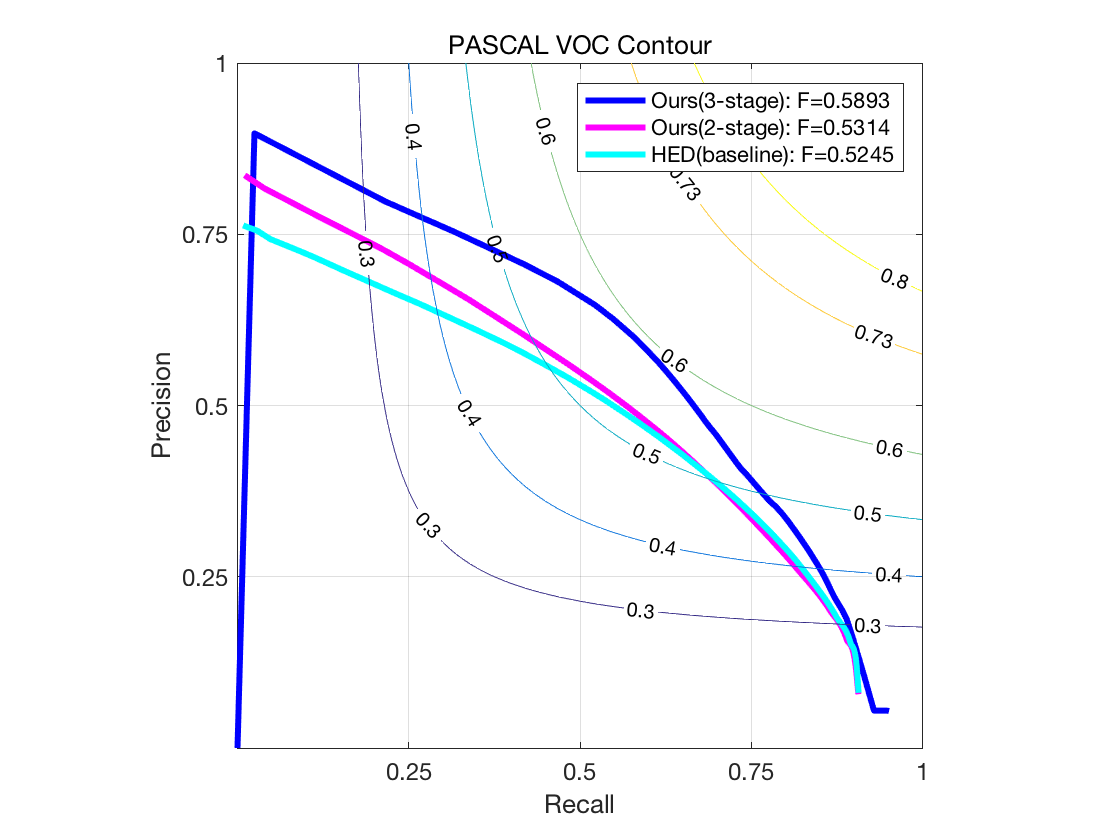
\includegraphics[width=15cm]{voc_prcurve.png}\\
  \caption{Precision-recall curves on PASCAL VOC Contour Dataset\cite{Yang2016}.}\label{voc prcurve}
\end{figure}

\section{Control Experiments for Model Interpretation}3

To verify the explaination and interpretation in Section \ref{interpretation}, we design a series of control experiments and give the neuronal boundary detection evaluation on Mouse Piriform Cortex Dataset\cite{Lee2015}. We do not test on the ISBI 2012 Segmentation Dataset\cite{Ronneberger2015} since there is no provided annotation for testing images on it. 

There are three control experiments, for which we design eight kind of networks with different network structures:

$\bullet$ \textbf{Baseline} HED\cite{Xie2015} pre-trained on BSDS 500 Dataset\cite{Arbelaez2011}

$\bullet$ \textbf{Nerwork A} 1-stage (HED\cite{Xie2015}) network with 5 levels in one stage, end-to-end training and no recursive input;

$\bullet$ \textbf{Network B} 2-stage cascaded network with 4 levels in each stage, end-to-end training and multi-recursive-input;

$\bullet$ \textbf{Network C} 2-stage cascaded network with 5 levels in each stage, end-to-end training and multi-recursive-input;

$\bullet$ \textbf{Network D} 3-stage cascaded network with 5 levels in each stage, end-to-end training and multi-recursive-input;

$\bullet$ \textbf{Network E} 2-stage cascaded network with 5 levels in each stage, end-to-end training and single-recursive-input (only the level 4);

$\bullet$ \textbf{Network F} 2-stage cascaded network with 5 levels in each stage, end-to-end training and single-recursive-input (only the level 5);

$\bullet$ \textbf{Network G} 2-stage cascaded network with 5 levels in each stage, stepwise training and multi-recursive-input;


\subsection{Evaluations on Cascaded Architecture \emph{vs.} Single-stage Architecture}

\begin{table}[t]
\renewcommand{\arraystretch}{0.6}
\caption{Control Experiment 1: Cascaded Architecture \emph{vs.} Single-stage Architecture}
\label{outcome}
\begin{center}
\begin{tabular}{|c|c|}
\hline
&\multicolumn{1}{c|}{Rand F-score}\\
\hline
Baseline 			& 0.9680	\\	\hline
Network A 		& 0.9688 	\\	\hline
Network B			& 0.9739	 \\	\hline
Network C 		& 0.9819	\\	\hline
Network D 		& 0.9866	\\	\hline
\end{tabular}
\end{center}
\label{control experiment 1}
\end{table}

To prove the proposed cascaded architecture effective in boundary detection, we compare our 2-stage (Network C) and 3-stage (Network E) cascaded networks with a 1-stage fine-tuned HED\cite{Xie2015} network (Network A) and the baseline HED\cite{Xie2015} pre-trained on a local edge boundary detection dataset, BSDS 500\cite{Arbelaez2011}. Results show that even a 2-stage cascaded network with only 4 convolution levels outperforms the baseline and the single-stage fine-tuned network with 5 convolution levels. If we stack more sub-networks while controlling the rest hyper-parameters, we can find the performance boosting from 0.9688 (Network A), to 0.9819 (Network C) and 0.9866 (Network D) step by step (Table \ref{control experiment 1}), which indicates that the proposed cascaded structures effective in high-level object boundary detection. The improvement achieved by stepwise removing the confounding local edges inside the objects (circuits), and refining the boundary with low contrast to the non-boundary area, illustrated by Fig. \ref{control 1}.

\begin{figure}[t]
  \centering
  % Requires \usepackage{graphicx}
  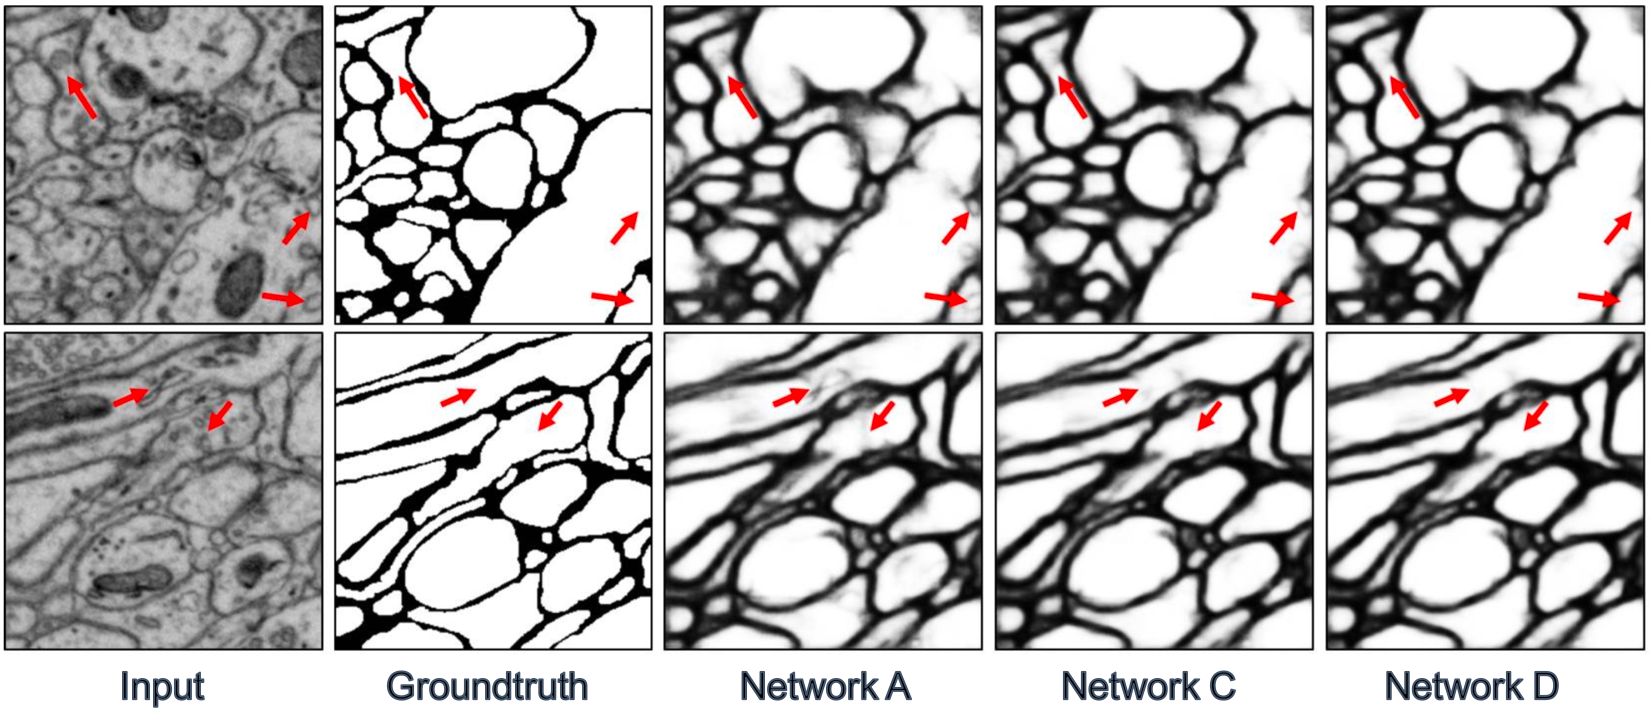
\includegraphics[width=15cm]{control_1.png}\\
  \caption{Qualitative examples to reveal how cascaded networks improve the high-level boundary detection result. For example, the arrows mean the false positive detections are removed step by step.}\label{control 1}
\end{figure}

\subsection{Evaluations on Multi-recursive-input vs. Single-recursive-input}

\begin{table}[t]
\renewcommand{\arraystretch}{0.6}
\caption{Control Experiment 2: Multi-recursive-input vs. Single-recursive-input}
\label{outcome}
\begin{center}
\begin{tabular}{|c|c|}
\hline
&\multicolumn{1}{c|}{Rand F-score}\\
\hline
Network F 		& 0.9410 	\\	\hline
Network E			& 0.9656	 \\	\hline
Baseline	 		& 0.9680	\\	\hline
Network C 		& 0.9819	\\	\hline
\end{tabular}
\end{center}
\label{control_experiment_2}
\end{table}

As we mentioned in Section {interpretation}, Multi-recursive-input plays a important role in the high-level object boundary detection, by providing the multi-scale features in a natural way. In order to evaluate it, we design several 2-stage single-recursive-input networks (Network E, F) and compare them with our 2-stage multi-recursive-input network (Network C). Cause we do not know which level is the best for inputing to the next stage, we input the level 4 (in Network E) and level 5 (in Network F) to the next sub-network respectively. According to Table \ref{control_experiment_2}, we surprisingly find the cascaded networks with single-recursive-input perform bad even when comparing with the pre-trained 1-stage network (Baseline). The single-recursive-input from the previous stage has only the features in one scale, either large or small. If we only feed the large-scale features with low-resolution into the next stage, there will be the a huge loss in image details. If we only feed the small-scale features into the next stage, the cascaded structure will be deprecated. It is always a hard problem for people to choose a best level as the recursive input, so we highlight the multi-recursive-input again in the cascaded structures.

\subsection{Evaluations on End-to-end Training vs. Stepwise Self-tuning}

\begin{table}[t]
\renewcommand{\arraystretch}{0.6}
\caption{Control Experiment 3: End-to-end Training vs. Stepwise Self-tuning}
\label{outcome}
\begin{center}
\begin{tabular}{|c|c|}
\hline
&\multicolumn{1}{c|}{Rand F-score}\\
\hline
Baseline	 		& 0.9680	\\	\hline
Network G 		& 0.9762	\\	\hline
Network C 		& 0.9819	\\	\hline
\end{tabular}
\end{center}
\label{control_experiment_3}
\end{table}

In the end, we design a control experiment with only the training strategy varied to see whether our cascaded networks benefit from the end-to-end training or not. As shown in Table \ref{control_experiment_3}, the cascaded network trained end-to-end (Network C) outperforms the same network but trained stepwise (Network G). The end-to-end training was hardly used to learn such a deep network, due to the consideration of gradient vanishing. However, the holistically-nested sub-networks and multi-recursive-input release the limitation, which enables the end-to-end training in our deep cascaded networks. 

\chapter{Conclusions} \label{conclusions}

Object-level boundary is a useful but unexplored topic in computer vision. With a well-detected object boundary, the segment of the object will be easily extracted, which can be applied for object proposal, shape based object recognition and  kinds of object detection problems. Based on the previous works in neuronal boundary detection, we develop a series of cascaded fully convolutional networks to detection high-level boundary in EM images. Not end up with the improvement achieved in EM images, we further extend the cascaded architecture to the object boundary detection in natural images, and design several control experiments to interpret how it works. Our model is proved to be both effective and interpretable in various boundary detection scenes, thus easy to be aggregated with other frameworks.

In the future, we will try some other structures for the alternative sub-networks, such as the recent published Richer Convolutional Features for Edge Detection\cite{Liu2017}, which is now the state-of-the-art on many edge detection benchmarks. Applications of our object-level boundary detection can be also considered, such as the boundary-based object proposal\cite{Yang2016}. 







\bibliographystyle{IEEEtran}
\bibliography{LUOreference}


\end{document}
